%%%%%%%% ICML 2022 EXAMPLE LATEX SUBMISSION FILE %%%%%%%%%%%%%%%%%

\documentclass[nohyperref]{article}

% Recommended, but optional, packages for figures and better typesetting:
\usepackage{microtype}
\usepackage{graphicx}
% \usepackage{subfigure}
\usepackage{booktabs} % for professional tables
\usepackage{enumitem,pifont}
\usepackage{subcaption}
%\usepackage{calrsfs}
%\DeclareMathAlphabet{\pazocal}{OMS}{zplm}{m}{n}
%\usepackage{mathrsfs}
%\usepackage[math-style=TeX, bold-style=TeX]{unicode-math}
%\setmathfont{XITS Math}
%\setmathfont[range={\mathscr,\mathbfscr,\mathcal,\mathbfcal}]{Cambria Math}
%\def\Lcs#1{\texttt{\textbackslash#1}}
% hyperref makes hyperlinks in the resulting PDF.
% If your build breaks (sometimes temporarily if a hyperlink spans a page)
% please comment out the following usepackage line and replace
% \usepackage{icml2022} with \usepackage[nohyperref]{icml2022} above.
\usepackage{hyperref}


% Attempt to make hyperref and algorithmic work together better:
\newcommand{\theHalgorithm}{\arabic{algorithm}}

% Use the following line for the initial blind version submitted for review:
\usepackage{icml2022}

% If accepted, instead use the following line for the camera-ready submission:
% \usepackage[accepted]{icml2022}

% For theorems and such
\usepackage{amsmath}
\usepackage{amssymb}
\usepackage{mathtools}
\usepackage{amsthm}

% if you use cleveref..
\usepackage[capitalize,noabbrev]{cleveref}

%%%%%%%%%%%%%%%%%%%%%%%%%%%%%%%%
% THEOREMS
%%%%%%%%%%%%%%%%%%%%%%%%%%%%%%%%
\theoremstyle{plain}
\newtheorem{theorem}{Theorem}[section]
\newtheorem{proposition}[theorem]{Proposition}
\newtheorem{lemma}[theorem]{Lemma}
\newtheorem{corollary}[theorem]{Corollary}
\theoremstyle{definition}
\newtheorem{definition}[theorem]{Definition}
\newtheorem{assumption}[theorem]{Assumption}
\theoremstyle{remark}
\newtheorem{remark}[theorem]{Remark}

% Todonotes is useful during development; simply uncomment the next line
%    and comment out the line below the next line to turn off comments
%\usepackage[disable,textsize=tiny]{todonotes}
\usepackage[textsize=tiny]{todonotes}
%\DeclareUnicodeCharacter{2212}{-}
% Defining mycomment
\newcounter{mycomment}
\newcommand{\mycomment}[2][]{%
% initials of the author (optional) + note in the margin
\refstepcounter{mycomment}{%\setstretch{0.7}
\todo[color={red!100!green!33}]{%
\textbf{Comment [\uppercase{#1}\themycomment]:}~#2}%
}}



\makeatletter
\if@todonotes@disabled
\newcommand{\hlfix}[2]{#1}
\else
\newcommand{\hlfix}[2]{\texthl{#1}\todo{#2}}
\fi
\makeatother



%%%%%%%%%%%%%%%%%%%%%%%%%%%%%%%%
% More space in the margins
%%%%%%%%%%%%%%%%%%%%%%%%%%%%%%%%

%\paperwidth=\dimexpr \paperwidth + 6cm\relax
%\oddsidemargin=\dimexpr\oddsidemargin + 3cm\relax
%\evensidemargin=\dimexpr\evensidemargin + 3cm\relax
%\marginparwidth=\dimexpr \marginparwidth + 3cm\relax
%\setlength{\marginparwidth}{ 3cm}


%%%%%%%%%%%%%%%%%%%%%%%%%%%%%%%%
% Graphics path 
%%%%%%%%%%%%%%%%%%%%%%%%%%%%%%%%
\graphicspath{{figures/}} 
% The \icmltitle you define below is probably too long as a header.
% Therefore, a short form for the running title is supplied here:
\icmltitlerunning{Submission and Formatting Instructions for ICML 2022}

\begin{document}

\twocolumn[
\icmltitle{Submission and Formatting Instructions for \\
           International Conference on Machine Learning (ICML 2022)}

% It is OKAY to include author information, even for blind
% submissions: the style file will automatically remove it for you
% unless you've provided the [accepted] option to the icml2022
% package.

% List of affiliations: The first argument should be a (short)
% identifier you will use later to specify author affiliations
% Academic affiliations should list Department, University, City, Region, Country
% Industry affiliations should list Company, City, Region, Country

% You can specify symbols, otherwise they are numbered in order.
% Ideally, you should not use this facility. Affiliations will be numbered
% in order of appearance and this is the preferred way.
\icmlsetsymbol{equal}{*}

\begin{icmlauthorlist}
\icmlauthor{Firstname1 Lastname1}{equal,yyy}
\icmlauthor{Firstname2 Lastname2}{equal,yyy,comp}
\icmlauthor{Firstname3 Lastname3}{comp}
\icmlauthor{Firstname4 Lastname4}{sch}
\icmlauthor{Firstname5 Lastname5}{yyy}
\icmlauthor{Firstname6 Lastname6}{sch,yyy,comp}
\icmlauthor{Firstname7 Lastname7}{comp}
%\icmlauthor{}{sch}
\icmlauthor{Firstname8 Lastname8}{sch}
\icmlauthor{Firstname8 Lastname8}{yyy,comp}
%\icmlauthor{}{sch}
%\icmlauthor{}{sch}
\end{icmlauthorlist}

\icmlaffiliation{yyy}{Department of XXX, University of YYY, Location, Country}
\icmlaffiliation{comp}{Company Name, Location, Country}
\icmlaffiliation{sch}{School of ZZZ, Institute of WWW, Location, Country}

\icmlcorrespondingauthor{Firstname1 Lastname1}{first1.last1@xxx.edu}
\icmlcorrespondingauthor{Firstname2 Lastname2}{first2.last2@www.uk}

% You may provide any keywords that you
% find helpful for describing your paper; these are used to populate
% the "keywords" metadata in the PDF but will not be shown in the document
\icmlkeywords{Machine Learning, ICML}

\vskip 0.3in
]

% this must go after the closing bracket ] following \twocolumn[ ...

% This command actually creates the footnote in the first column
% listing the affiliations and the copyright notice.
% The command takes one argument, which is text to display at the start of the footnote.
% The \icmlEqualContribution command is standard text for equal contribution.
% Remove it (just {}) if you do not need this facility.

%\printAffiliationsAndNotice{}  % leave blank if no need to mention equal contribution
\printAffiliationsAndNotice{\icmlEqualContribution} % otherwise use the standard text.

\begin{abstract}
This document provides a basic paper template and submission guidelines.
Abstracts must be a single paragraph, ideally between 4--6 sentences long.
Gross violations will trigger corrections at the camera-ready phase.
\end{abstract}

\section{Introduction}

    Neural networks have become the \textit{de facto} approach for many if not
    all machine learning applications \cite{lecunDeepLearning2015}, from  image
    recognition \cite{dengImageNetLargescaleHierarchical2009} to  natural language
    processing \cite{devlinBERTPretrainingDeep2019} and  
    speech synthesis \cite{oordWaveNetGenerativeModel2016}.
    Given their heavy reliance on increasing computing and memory
    \cite{brownLanguageModelsAre2020,thompsonComputationalLimitsDeep2020}
    methods for compressing networks but that retain performance has become
    increasingly popular.

Neural Network pruning is a popular compression technique that consist in the
removal of weights while retaining good performance.
Most approaches currently used try to identify a subset of weights from a
pretrained reference network either via a saliency criteria
\cite{mozerSkeletonizationTechniqueTrimming1988,
hassibiSecondOrderDerivatives1992,lecunOptimalBrainDamage1989} or by
regularization during training
\cite{chauvinBackPropagationAlgorithmOptimal1988,
carreira-perpinanLearningCompressionAlgorithmsNeural2018}. All of these
approaches, however, need several expensive prune-retrain cycles and heuristic
design decisions with extra hyperparameters making it difficult to adapt them
to new architectures and task.

In this paper we propose a simple pruning procedure that do not need
fine-tuning for retaining accuracy. Our method, named \textit{stochastic
pruning}, uses only inference and stochastic perturbation of weights in an
iterative manner.
Our contributions are:
     \begin{itemize}
         \item We shed light into the phenomena that stochastic pruning is not
             only feasible but also can outperform deterministic pruning
             reliably.
         %\item  We characterized this phenomena in terms of its hyperparameters namely the population size $N$ and the noise variance $\sigma$
        \item An iterative stochastic pruning algorithm that achieves minimum
            accuracy loss without fine tuning

        \item We uncover the existence of ``motifs'' in parameter heavy
                layers after massively pruning them, showing that pruning
                improves the explainability (clusterability) of
                networks.\todo{Still not sure about this}

     \end{itemize}
     
We perform  stochastic pruning on ResNet18, EfficientNet on CIFAR10,CIFAR100,
and ImageNet. Demostrating that our method is achieves good performance
without fine-tuning \todo{Here I should fine-tune deterministic pruning to
compare to my population algorithm.}

%This paper is 


%    This success is
%    reliant on the ever increasing availability of data and computing power
%    that researchers have used to train large state-of-the-art models
%    \cite{}. Due to the environmental and financial
%    concerns \cite{thompsonComputationalLimitsDeep2020}
%there has been an increasing interest in methods that lessen the computational
%burden of training and deploying these models. 


%Neural Network pruning is a popular compression technique for network
%compression.

%Magnitude based pruning \cite{hanLearningBothWeights2015a}

    The most popular method for neural network pruning is \textbf{magnitude
    pruning}  which despite of its simplicity  it has been proven to be competitive against more complex pruning
    strategies across datasets and architectures
    \cite{guptaComplexityRequiredNeural2022}. Despite that the solution found
    by Stochastic Gradient Descent at the end of training has the potential of
    being a global minima \cite{leeGradientDescentOnly2016,luDepthCreatesNo2017,
    zhouSGDConvergesGlobal2018,kawaguchiDeepLearningPoor2016} in general this
    is not the case \cite{dingSubOptimalLocalMinima2020}. Inspired by
    the

    %\mycomment[LUIS]{Here I was thinking on using the original argument we had that was to discover ``core'' connections and ``variable'' connections. That is how the idea of stochastic pruning came to be. But I felt that given the scope of the paper now. Introducing such idea is more difficult, maybe if I change the tone of the introduction or the motivation}



%
%intuition of the Optimal
%Brain Surgeon \cite{hassibiSecondOrderDerivatives1992}
%    where they suggested that an pruning strategy based on a quadratic
%    approximation of the loss function would suggest that the best pruning
%    strategy is no the one that removes the smallest weights but also the one
%    that rescales the weights accordingly. This
%    suggest that when projecting the full dense solution into a constrained
%    space e.g. prune, maybe eliminating the smallest dimensions is not
%    the best strategy.\todo{This does not make much sense since we are still using
%magnitude pruning but in a noisy model. So we are actually doing the same but
%on a different set of weights we just need  to motivate this differently}
%
%\vspace{3cm}
%\textbf{Outline of the  introduction}
%
%\begin{enumerate}
%    \item Neural networks are very popular in many areas of machine learning
%    \item The reason that this models are so popular now is due to the increase
%        in data and computation.
%    \item Neural network pruning is a popular option for reducing the computing
%        and memory footprint out of these increasingly large models
%    \item Magnitude pruning is a simple yet effective way of reducing size of
%        neural networks
%%    \item In order for a pruning algorithm algorithm to be effective it needs
%        to identify the less relevant weights in the network
%    % \item Inspired from the fact that C. elegans worms have a \textbf{core}
%    %     neural circuit that is common among the whole species and a \textbf{variable}
%    %     neural circuit that is particular individual, we believe that
%    %     inspecting differently pruned networks we can identify such core for a
%    %     particular architecture.
%    \item What we found is that with a small amplitude noise added to a
%        particular solution we can find different pruned solutions that can
%        outperform the orinal solution pruned.
%    \item This stochastic pruning is proved to be an inexpensive alternative
%        to deterministic pruning where without any fine-tuning is capable of
%        finding good solutions for high sparsity regimes.
%    \item We propose an iterative algorithm for obtaining a population of  pruned
%        networks that obtain good performing sparse networks without expensive
%        retraining.
%        
%
%    \item The contributions of this paper are as follows:
%     \begin{itemize}
%         \item We shed light into the phenomena that stochastic pruning is not
%             only feasible but also can outperform deterministic pruning
%             reliably.
%         %\item  We characterized this phenomena in terms of its hyperparameters namely the population size $N$ and the noise variance $\sigma$
%        \item An iterative stochastic pruning algorithm that achieves minimum
%            accuracy loss without fine tuning
%
%        \item We uncover the existence of ``motifs'' in parameter heavy
%                layers after massively pruning them, showing that pruning
%                improves the explainability of networks.\todo{I think I need
%            to rephrase this }
%
%     \end{itemize}
%
%\end{enumerate}
%    
%
%
%
%
%
%    In this work we use the widely used magnitude pruning and show that injecting small amounts of noise to a well
%    trained network we can obtain pruned networks that  outperform the original
%    ``clean'' model pruned.
   % Our experiments show how the drop in performance of
   % the noisy models depends on the number of noisy samples we draw and what are reasons why
   % this noisy pruned models can outperform deterministic pruning.

%    \textbf{Motivation:} The two main question with this phenomena is:
%    Do this stochastic models outperform the deterministic pruning due to the
%    mask they unveil? Or are the weighs themselves that drive the performance
%    gain?
%








%    But this success comes with exponential
%    growth in computation and storage needed for. The most common mechanism for
%    Neural network pruning has been widely studied in recent years as a way of addressing this issue



\section{Related work}
%\subsection{Outline}
% \begin{itemize}
%     \item There has been many research about neural network pruning and sparsity:

% \item         Some of the use second order
%         \cite{singhWoodFisherEfficientSecondOrder2020,
%         yuHessianAwarePruningOptimal2022}

%     \item  Some of them before training \todo{cite snip grasp and synflow} but they
%         cannot reach the same performance as post training pruning
%         \cite{franklePruningNeuralNetworks2021}.
%     \item There is another branch that is dynamical sparse training, where the mask is constantly changing  during the course of training \todo{Cite Riging the lottery, Evolutionary sparse training ,DEEP R, and many others I have in my zotero}    
    
% \end{itemize}

Neural network pruning can be grouped into \textit{After training pruning}
and  \textit{Pre-training } 
Also in this section we mention \textit{dynamical sparse training} were the
network's
connectivity  is also updated during training to obtain a good performing sparse network.

\textbf{Prunning After Training:} These methods prune a pre-trained network.
Each method has a different importance score to detect unimportant weights.
The most simple one is the magnitude of a weight
\cite{hanLearningBothWeights2015a,hanDeepCompressionCompressing2016a} where
weights with the lowest magnitude are deemed as
 unnecessary. However this method can remove important low magnitude weights.
 Some methods use the first order (i.e. gradient information) Taylor expansion
 coefficients of the loss function\cite{karninsimpleprocedurepruning1990a,mozerskeletonizationtechniquetrimming1988}.
 Hessian-based methods measure the importance of weights as the effect they
 have in the second order approximation of the final loss function 
 \cite{hassibiSecondOrderDerivatives1992,lecunOptimalBrainDamage1989,
 hassibiOptimalBrainSurgeon1993,singhWoodFisherEfficientSecondOrder2020}.
 Many of this methods require a fine-tuning phase to mitigate the accuracy
 drop.




\textbf{Pre-Training Pruning:} This family of algorithms prune a
network before training takes place on the randomly initialized weights. SynFlow
\cite{tanakaPruningNeuralNetworks2020a} uses a measure based on path-norm
\cite{neyshaburPathSGDPathNormalizedOptimization2015} that the authors call
synaptic flow which they prove avoids layer-collapse, this method do not use
data for pruning. Gradient Signal Preservation
(GrasP) \cite{wangPickingWinningTickets2020} prunes the randomly initialized network such that the
gradient flow signal is preserved through the network.
Lastly, Single-Shot Network Pruning Based on Connection Sensitivity
\cite{leeSNIPSINGLESHOTNETWORK2018} add parameters that represent the
connections (but not the weight) between neurons and uses the approximate
gradient of the loss function with respect to the new parameters as the
saliency score for pruning. 

\textbf{Dynamical Sparse Training:} In this category methods instead of
pruning once and leaving the mask static, they alter the mask during the
course of training which results in similar or better performance than the
dense counterparts.
This idea was first used in Sparse
Evolutionary Training (SET) \cite{mocanuScalableTrainingArtificial2018a} were
they initialized the network in a sparse manner and after
each epoch  a fraction of the weights closest to zero is pruned and the same
number of weights is grown back randomly.
Sparse Networks from Scratch (SNFS) \cite{dettmersSparseNetworksScratch2019}
regrowth method is based on the momentum of each weight, reallocating the weights from less efficient layers and redistribute them to weight-efficient layers.
Rigging the Lottery (RigL)  \cite{evciRiggingLotteryMaking2020}h strategy is to use the
"would be" gradients of the pruned parameters as the indicator for
incorporating new weights to the network. Deep R
\cite{bellecDeepRewiringTraining2018} uses a probabilistic framework for
regrowing and pruning connections on the network alongside to adding a random
walk to SGD in parameter space.

\section{Neural Network Pruning}



The primary premise neural network pruning is that since neural networks are frequently overparametrized, it is possible to achieve equal performance with a substantially smaller network \cite{reedPruningAlgorithmsaSurvey1993}, while enhancing generalisation.
To achieve this, then the objective is to find a sparse network that maintains
the performance of the over parametrized network. Then following the
formulation of neural network pruning as an optimization problem of
\cite{leeSNIPSINGLESHOTNETWORK2018}. Given a dataset $\mathcal{D}=\{(x_i,y_i)\} _{i=1}^{n}$
and a desired pruning level $\kappa$ (i.e., the number of zero weights) then
the optimization problem for neural network pruning can be stated as:
\begin{equation}
     \centering
    \begin{aligned}
          \underset{\mathbf{w,m}}{\min}\quad&  \frac{1}{n} \sum_{i=1}^{n}
          \ell(F(\mathbf{m}\odot \textbf{w};x_i),y_i)     \\
    \label{eq:pruning_optim_problem}
           s.t.\quad & \mathbf{w}\in \mathbb{R}^d\\
           \quad & \mathbf{m}\in \{0,1\}^d\quad \|\mathbf{m}\|_0 \geq \kappa
       \end{aligned}
\end{equation}
           where $\ell(\cdot)$ is the loss function, $\odot$ is the
           Hadamard product, $F(\mathbf{m}\odot \textbf{w};x)$ is the output
           of the neural network given the set of weights and masks, $d$ is the total number of
           parameters and $\|\cdot\|_0$ is the $L_0$ norm.
Most of the after-training pruning methods unveil a mask $m$ that is
static and fine-tune the remaining weights $\tilde{\mathbf{w}}=\mathbf{m}
\odot\mathbf{w}$ to minimize the accuracy drop, $\epsilon= ACC(\mathbf{w^*})
-ACC(\mathbf{\tilde{w}})$. This operation is expensive, since gradients need to be calculated for
the whole training dataset and in general they are calculated in a dense
manner (even when weights are 0 they are still used in the Backward pass). 



In this work we propose an gradient free population based iterative algorithm
that minimizes $\epsilon$. Our approach is more efficient than fine tuning and
is very simple to implement.
\section{Experiments}
We use a ResNet18 \cite{heDeepResidualLearning2015} trained for 200 epoch with
SGD, initial learning rate of  0.1, Cosine Annealing schedule with $T_{max}=200$ and batch size of 128.
We first shed light into fact that in the one-shot no fine-tuning regime
additive noise with magnitude pruning can reveal good performing subnetworks.
Based on this we propose an population based algorithm that recovers accuracy
without fine-tuning


\begin{equation}
\epsilon= \text{accuracy}_{\text{dense deterministic model}}-\text{accuracy}_{\text{pruned model}}
\end{equation}

\subsection{Unveiling Good Sparse Solutions without Training}
In this section we show an strange phenomenon that we detect on convolutional networks.  
We add Gaussian noise to our pretrained network with a set global noise level (standard deviation) $\sigma$ followed by standard Magnitude Pruning \cite{citeNeedCitation200007}. 
\begin{figure}
    \centering
    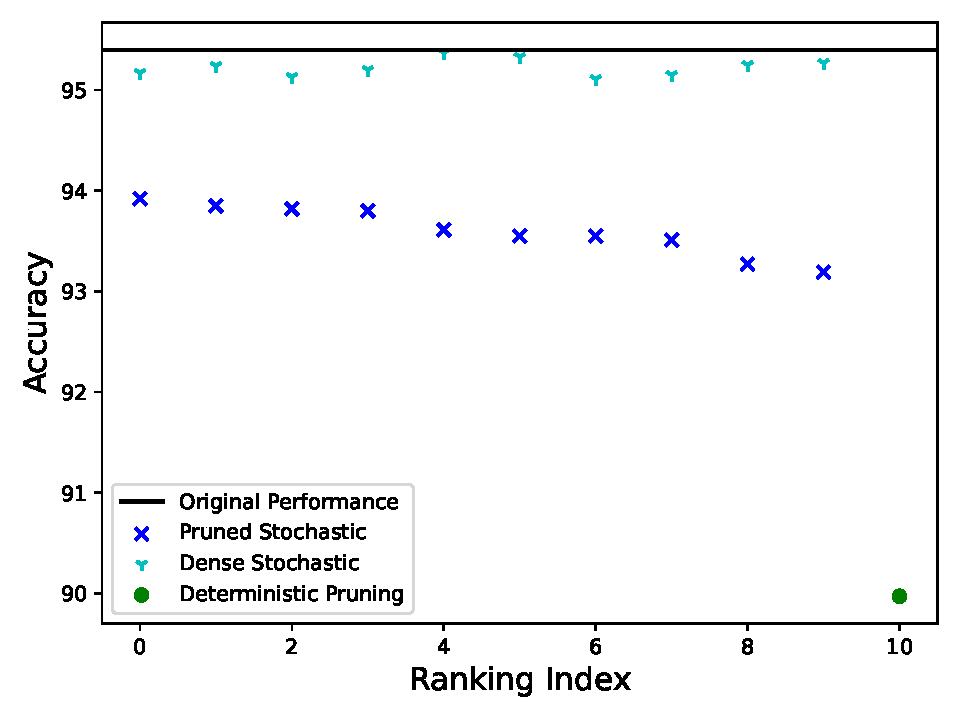
\includegraphics[width=0.45\textwidth]{figures/stochastic_deterministic_gaussian_sigma_0.002_pr_0.8_batchSize_512_pop_10_t_11-44_test.pdf}
    \caption{ Accuracy of one-shot pruned ResNet18 with 80\% sparsity in the CIFAR10 test set with $\sigma = 0.002$. In this case, 10 noisy samples were retrieved. Note that all dense noisy ResNet18 networks do not outperform the noiseless 
    original solution}
    \label{fig:stochastic_versus_deterministic}
\end{figure}

\begin{table}[!htb]
    \centering
    \caption{Median of weight magnitude per layer}
    \begin{tabular}{|l|l|}
    \hline
        \textbf{Layer Name} & \textbf{Median} \\ \hline
        conv1 & 5.29E-06 \\ \hline
        layer1.0.conv1 & 3.99E-07 \\ \hline
        layer1.0.conv2 & 5.41E-03 \\ \hline
        layer1.1.conv1 & 4.85E-03 \\ \hline
        layer1.1.conv2 & 4.24E-03 \\ \hline
        layer2.0.conv1 & 7.91E-03 \\ \hline
        layer2.0.conv2 & 7.53E-03 \\ \hline
        layer2.0.shortcut.0 & 1.17E-02 \\ \hline
        layer2.1.conv1 & 4.71E-03 \\ \hline
        layer2.1.conv2 & 4.39E-03 \\ \hline
        layer3.0.conv1 & 7.37E-03 \\ \hline
        layer3.0.conv2 & 6.74E-03 \\ \hline
        layer3.0.shortcut.0 & 9.55E-03 \\ \hline
        layer3.1.conv1 & 5.59E-03 \\ \hline
        layer3.1.conv2 & 4.07E-03 \\ \hline
        layer4.0.conv1 & 4.01E-03 \\ \hline
        layer4.0.conv2 & 2.24E-03 \\ \hline
        layer4.0.shortcut.0 & 4.41E-03 \\ \hline
        layer4.1.conv1 & 1.31E-03 \\ \hline
        layer4.1.conv2 & 7.08E-04 \\ \hline
        linear & 5.35E-02 \\ \hline
    \end{tabular}
    \label{tab:Q50perLayer}
\end{table}




% ####################################### Epsilon plotss##########################################
   
  % \begin{figure}[!htb]
  %   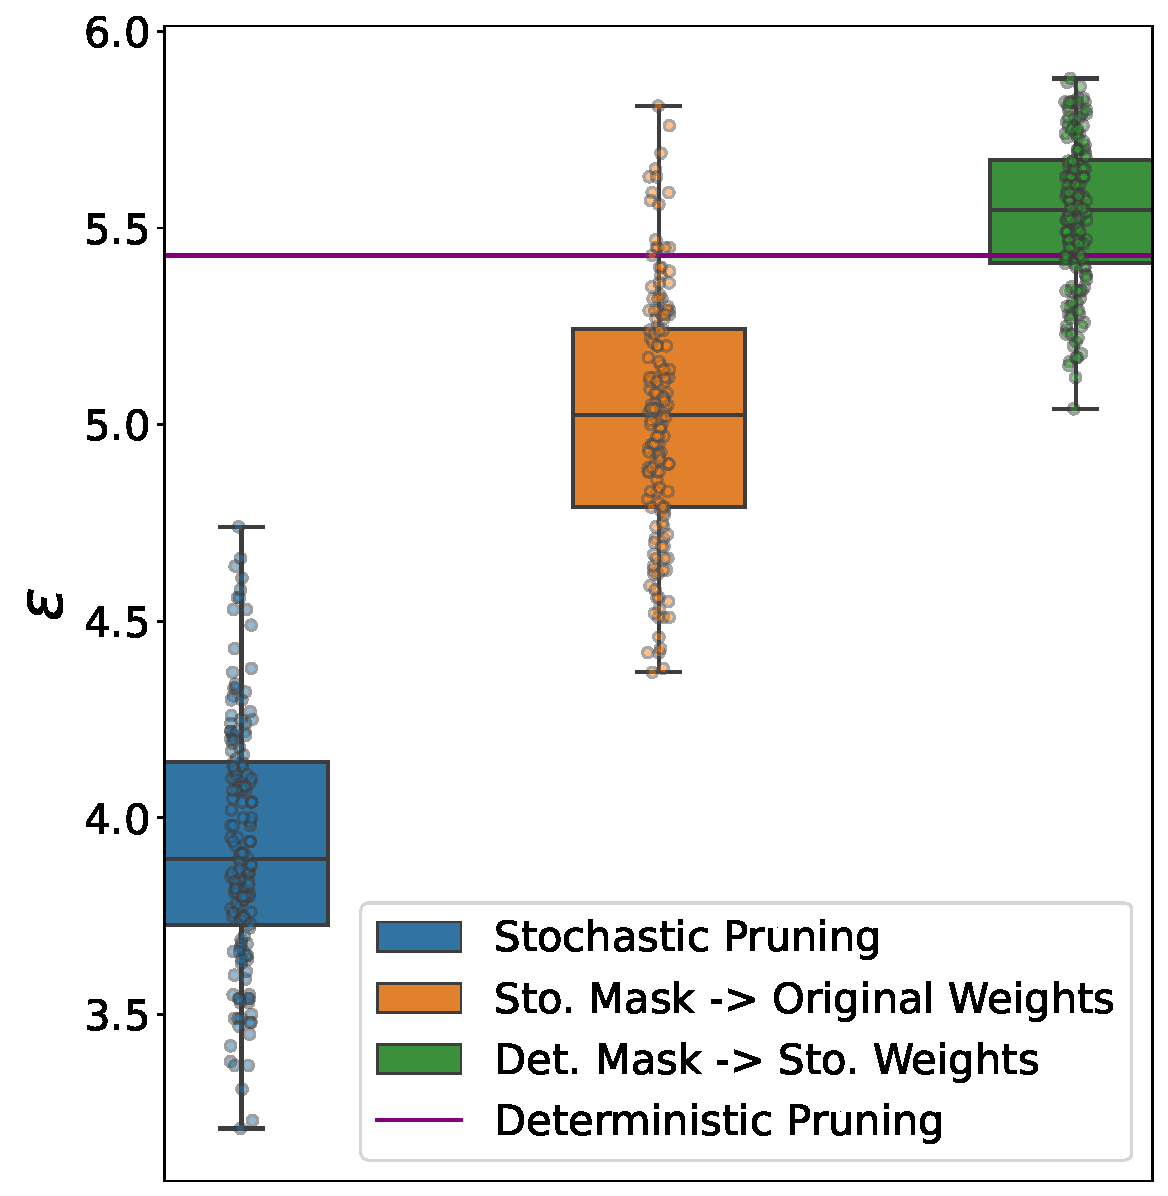
\includegraphics[width=\columnwidth]{figures/epsilon_allN_all_pr_0.8_sigma=0.001.pdf}
  %   \caption{Accuracy degradation of One-shot Stochastic Pruning with $\sigma=0.001$ and pruning rate of 0.8} \label{fig:pr0.8sigma0.001}
  % \end{figure}%
  % \begin{figure}[!htb]
  %   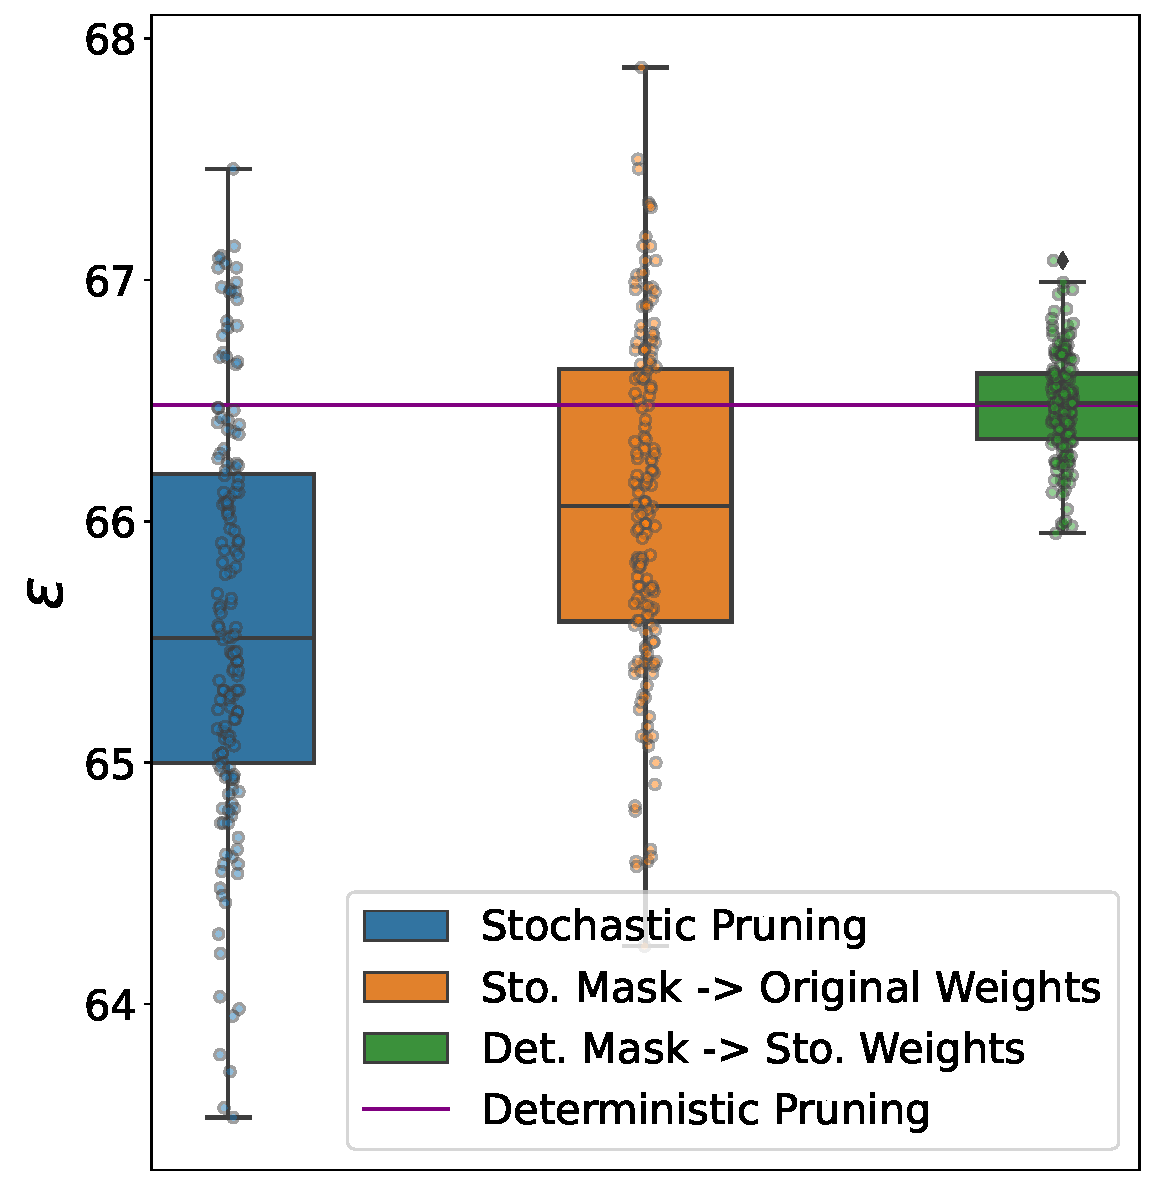
\includegraphics[width=\columnwidth]{figures/epsilon_allN_all_pr_0.9_sigma=0.001.pdf}
  %   \caption{Accuracy degradation of One-shot Stochastic Pruning with $\sigma=0.001$ and pruning rate of 0.9} \label{fig:pr0.9sigma0.001}
  % \end{figure}%



  % \begin{figure}[!htb]
  %   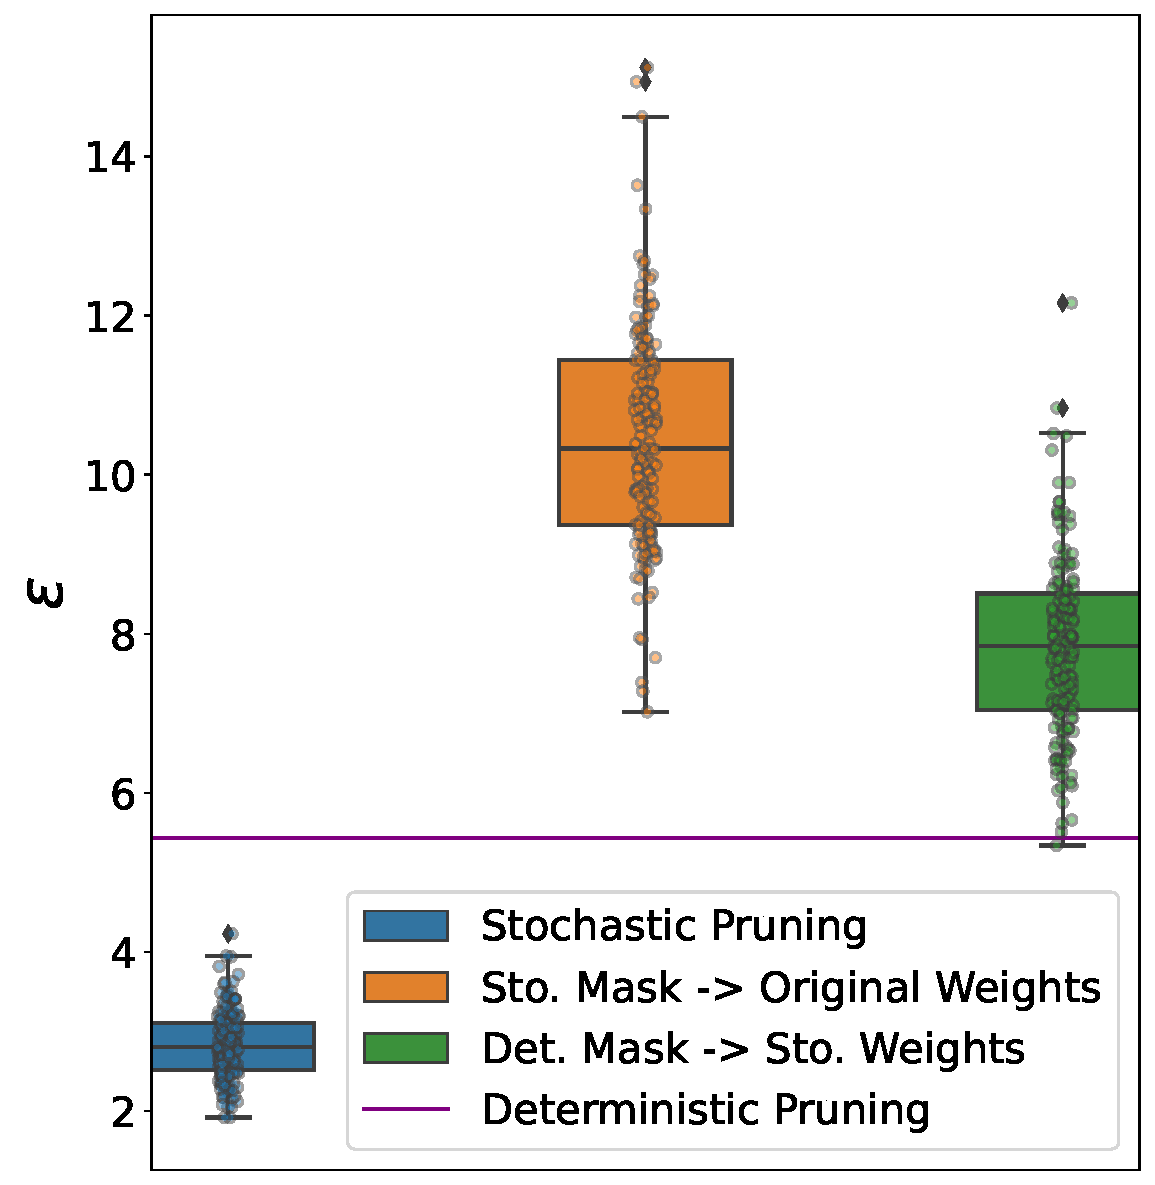
\includegraphics[width=\columnwidth]{figures/epsilon_allN_all_pr_0.8_sigma=0.005.pdf}
  %   \caption{Accuracy degradation of One-shot Stochastic Pruning with $\sigma=0.005$ and pruning rate of 0.8} \label{fig:pr0.8sigma0.005}
  % \end{figure}

  % \begin{figure}[!htb]
  %   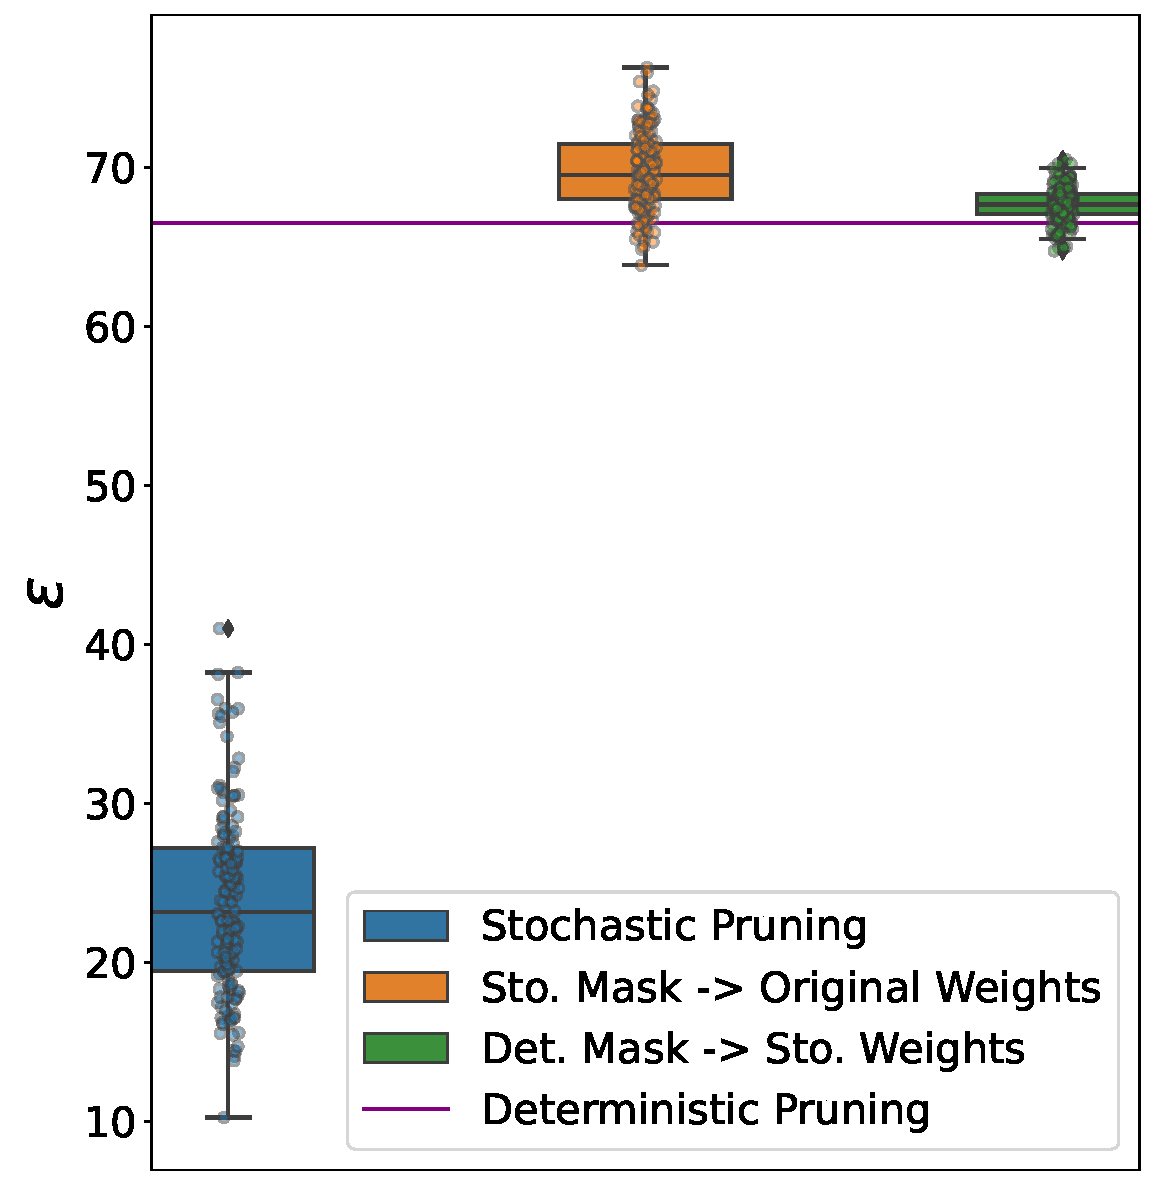
\includegraphics[width=\columnwidth]{figures/epsilon_allN_all_pr_0.9_sigma=0.005.pdf}
  %   \caption{Accuracy degradation of One-shot Stochastic Pruning with $\sigma=0.005$ and pruning rate of 0.9} \label{fig:pr0.9sigma0.005}
  % \end{figure}

\begin{figure*}[!htb]
  \centering
     \begin{subfigure}[b]{0.65\columnwidth}
         \centering
    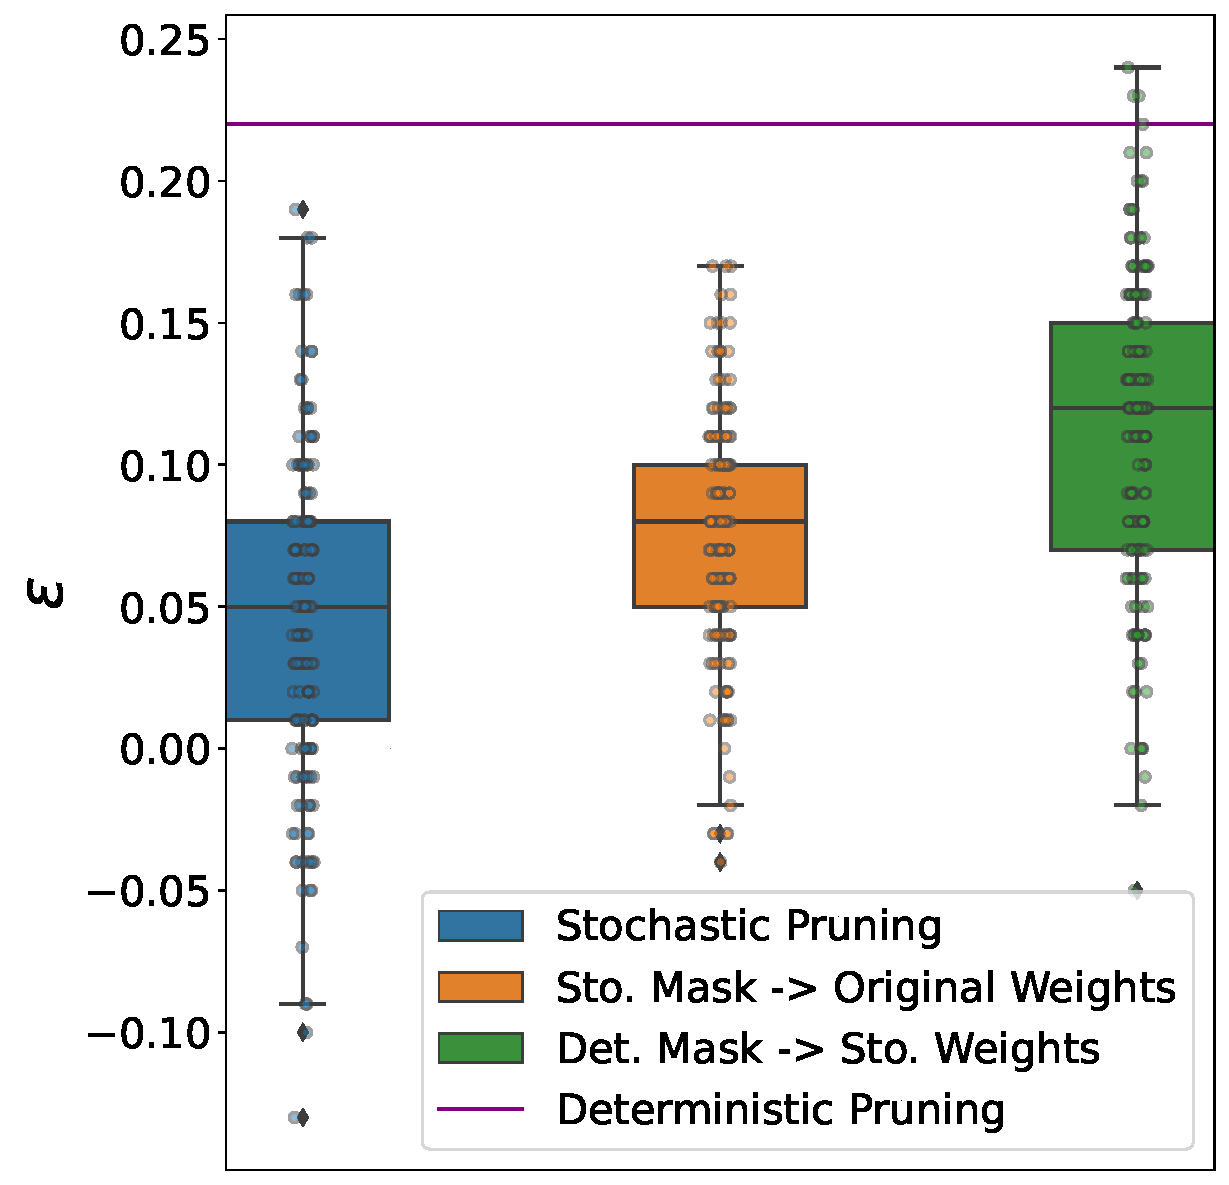
\includegraphics[width=\columnwidth]{figures/epsilon_allN_all_pr_0.5_sigma=0.001.pdf}
    % \caption{Accuracy degradation of One-shot Stochastic Pruning with $\sigma=0.001$ and pruning rate of 0.5} 
    \caption{ Pruning rate 0.5} 
    \label{fig:pr0.5sigma0.001}
     \end{subfigure}
     \hfill
     \begin{subfigure}[b]{0.65\columnwidth}
         \centering
   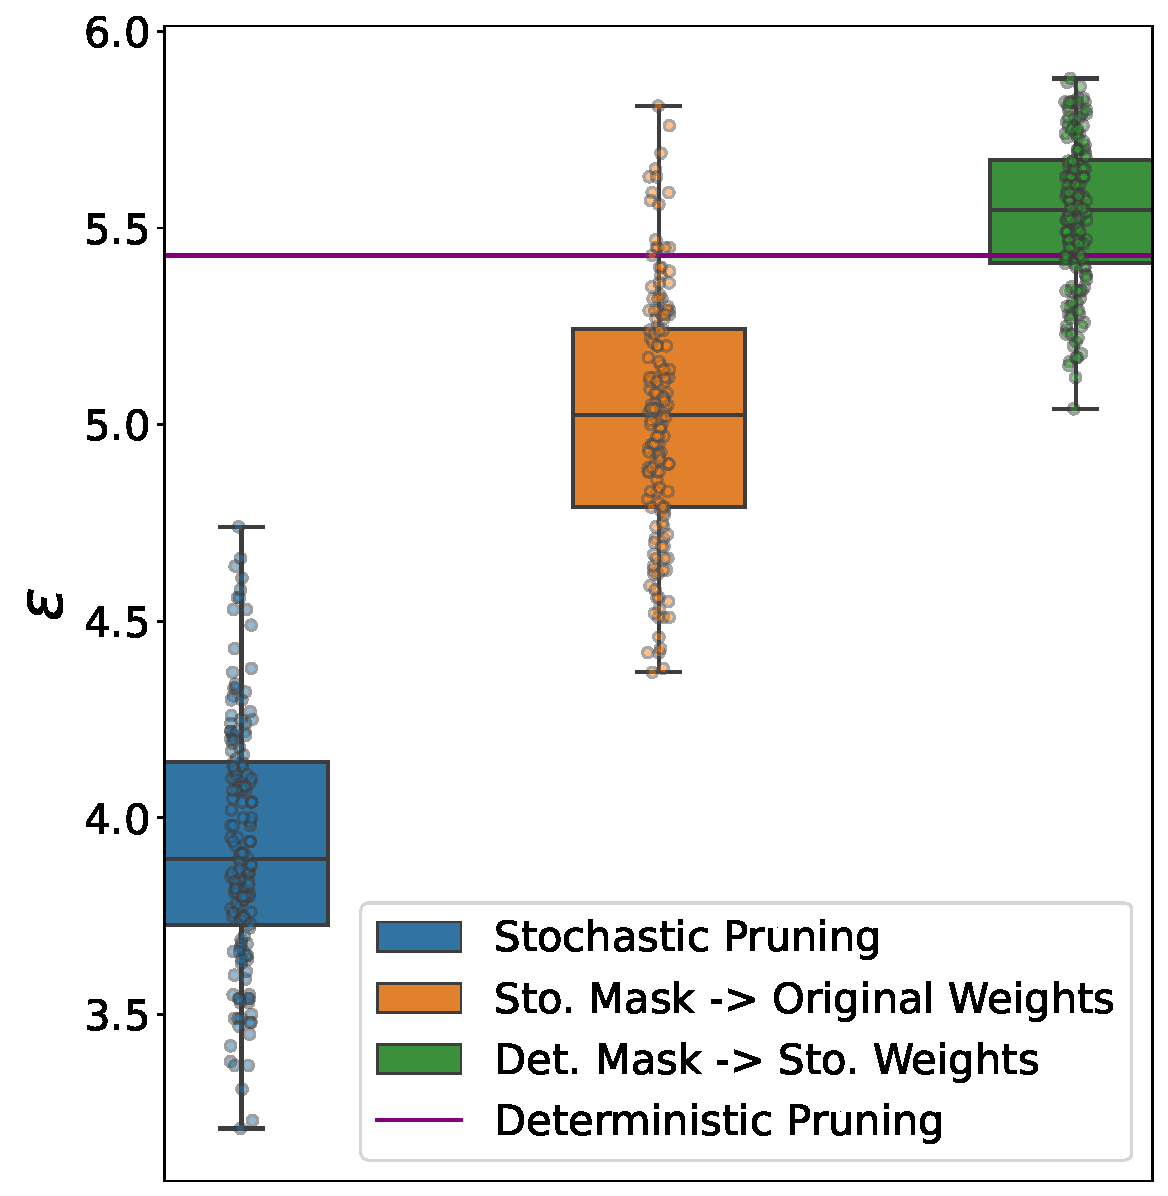
\includegraphics[width=\columnwidth]{figures/epsilon_allN_all_pr_0.8_sigma=0.001.pdf}
   
    \caption{ Pruning rate 0.8} 
    \label{fig:pr0.8sigma0.001}
     \end{subfigure}
    \hfill
     \begin{subfigure}[b]{0.65\columnwidth}
         \centering
     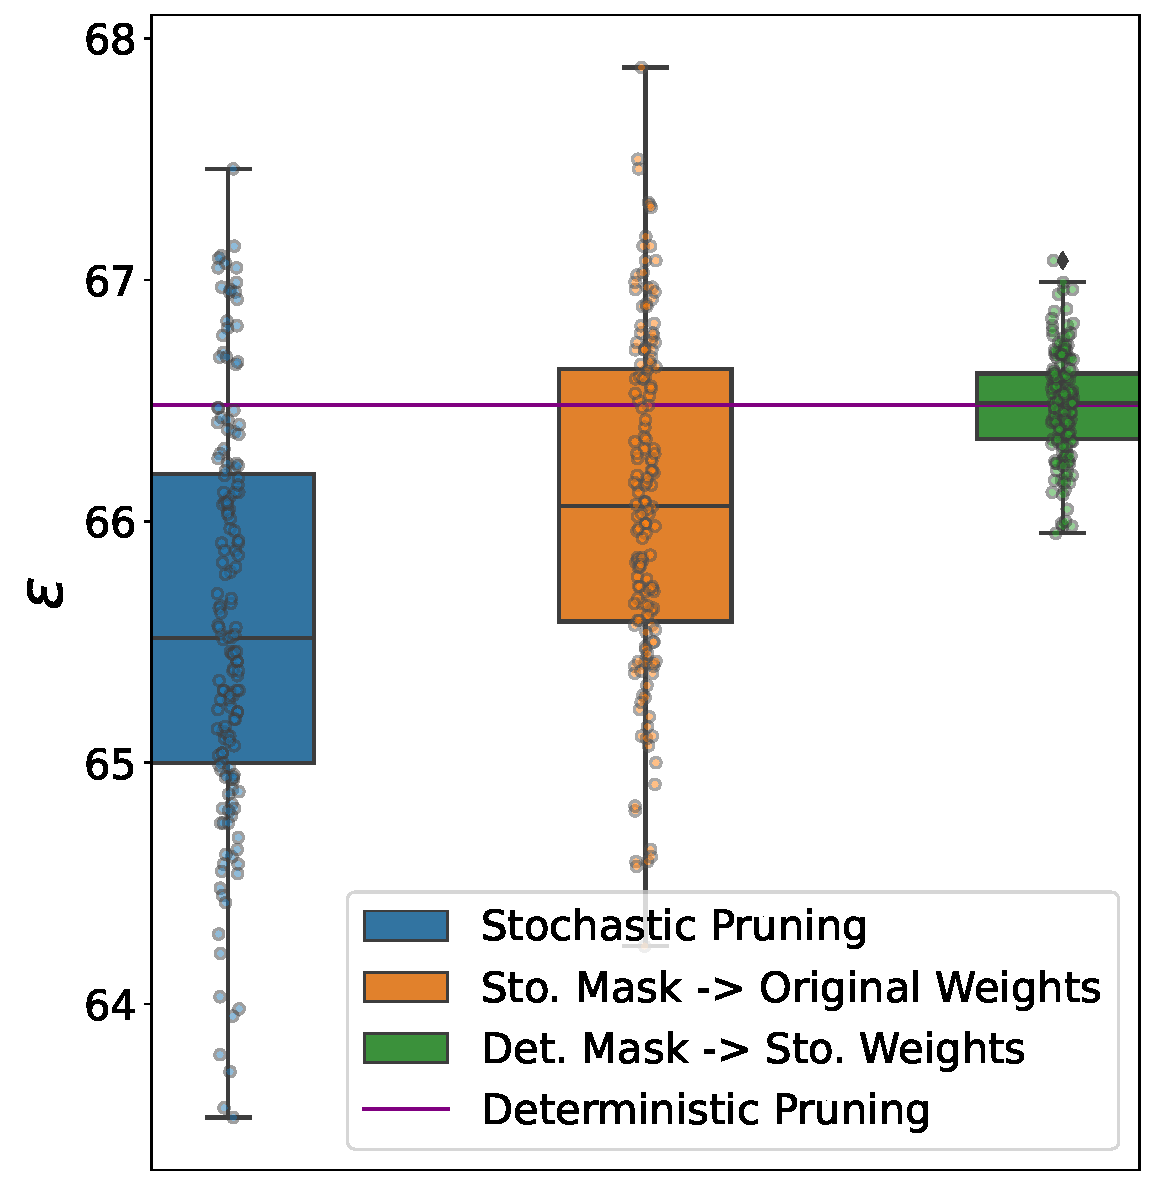
\includegraphics[width=\columnwidth]{figures/epsilon_allN_all_pr_0.9_sigma=0.001.pdf}
    % \caption{Accuracy degradation of One-shot Stochastic Pruning with $\sigma=0.001$ and pruning rate of 0.9} 
    \caption{ Pruning rate 0.9} 
    \label{fig:pr0.9sigma0.001}
     \end{subfigure}
     \caption{Accuracy degradation of One-shot Stochastic Pruning and the resulting models of operations \ref{operation1} and \ref{operation2} with $\sigma=0.001$}
     \label{fig:sigma0.001}
\end{figure*}

\begin{figure*}[!htb]
  \centering
     \begin{subfigure}[b]{0.65\columnwidth}
         \centering
    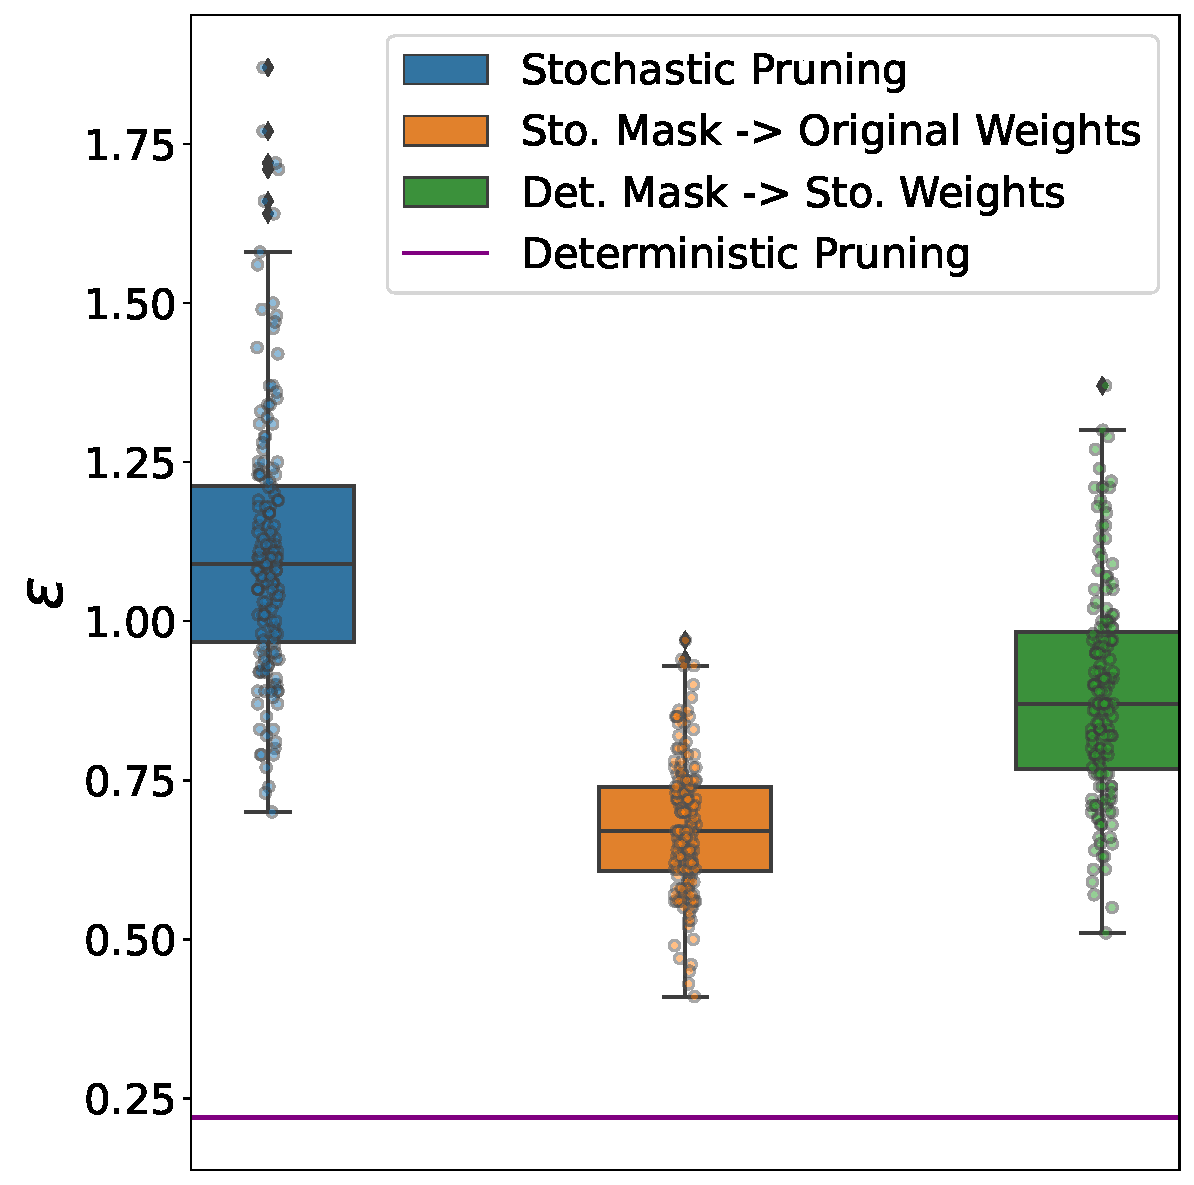
\includegraphics[width=\columnwidth]{figures/epsilon_allN_all_pr_0.5_sigma=0.005.pdf}
    % \caption{Accuracy degradation of One-shot Stochastic Pruning with $\sigma=0.001$ and pruning rate of 0.5} 
    \caption{Pruning rate 0.5} 
    \label{fig:pr0.5sigma0.005}
     \end{subfigure}
     \hfill
     \begin{subfigure}[b]{0.65\columnwidth}
         \centering
   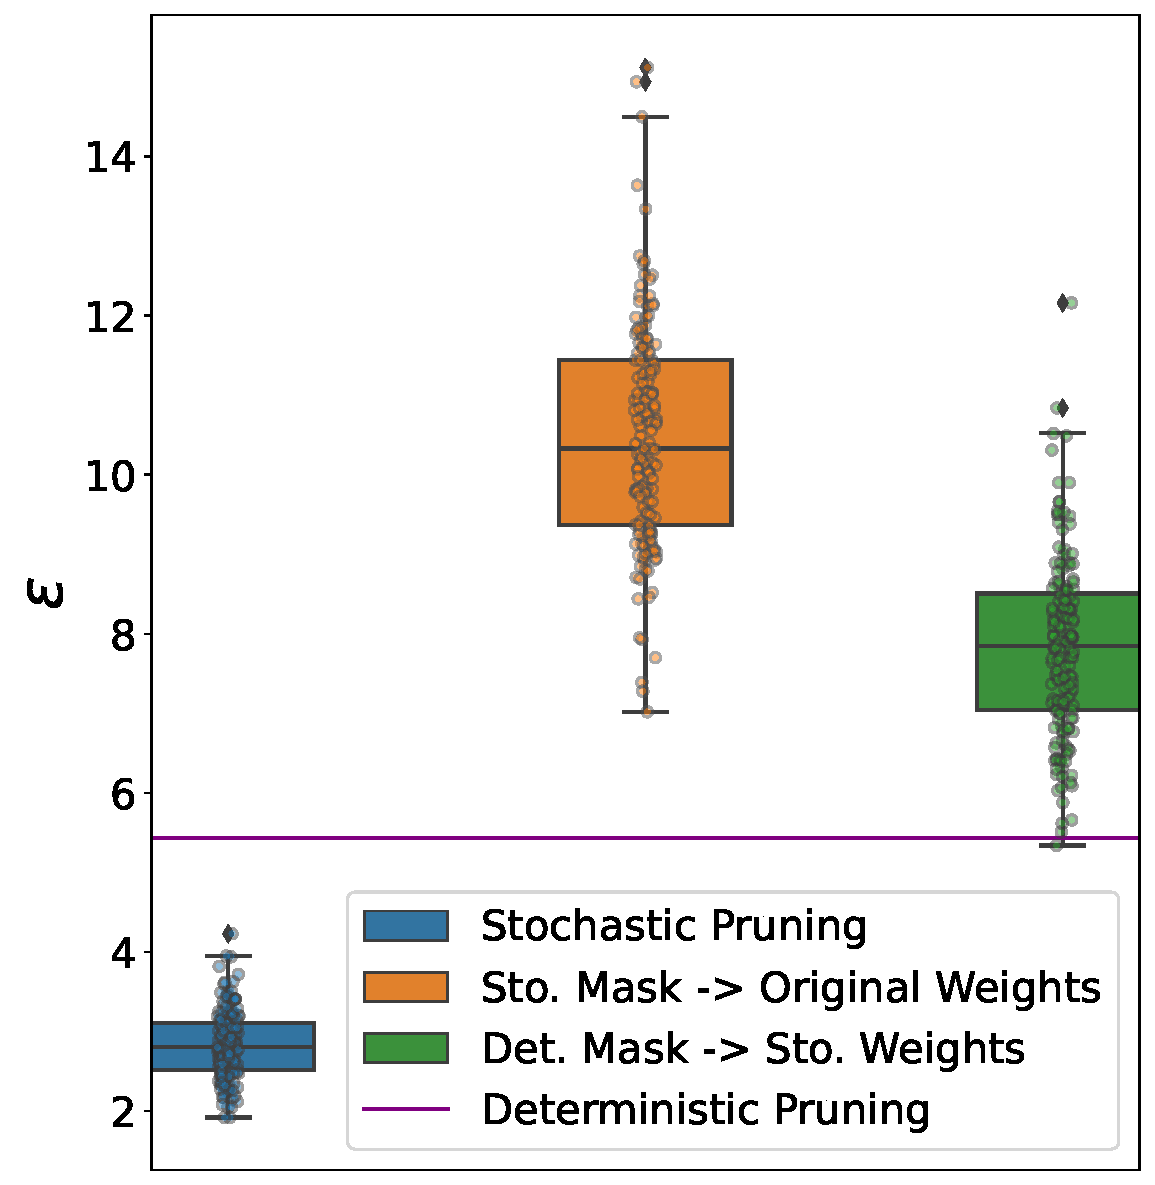
\includegraphics[width=\columnwidth]{figures/epsilon_allN_all_pr_0.8_sigma=0.005.pdf}
   
    \caption{Pruning rate 0.8} 
    \label{fig:pr0.8sigma0.005}
     \end{subfigure}
    \hfill
     \begin{subfigure}[b]{0.65\columnwidth}
         \centering
     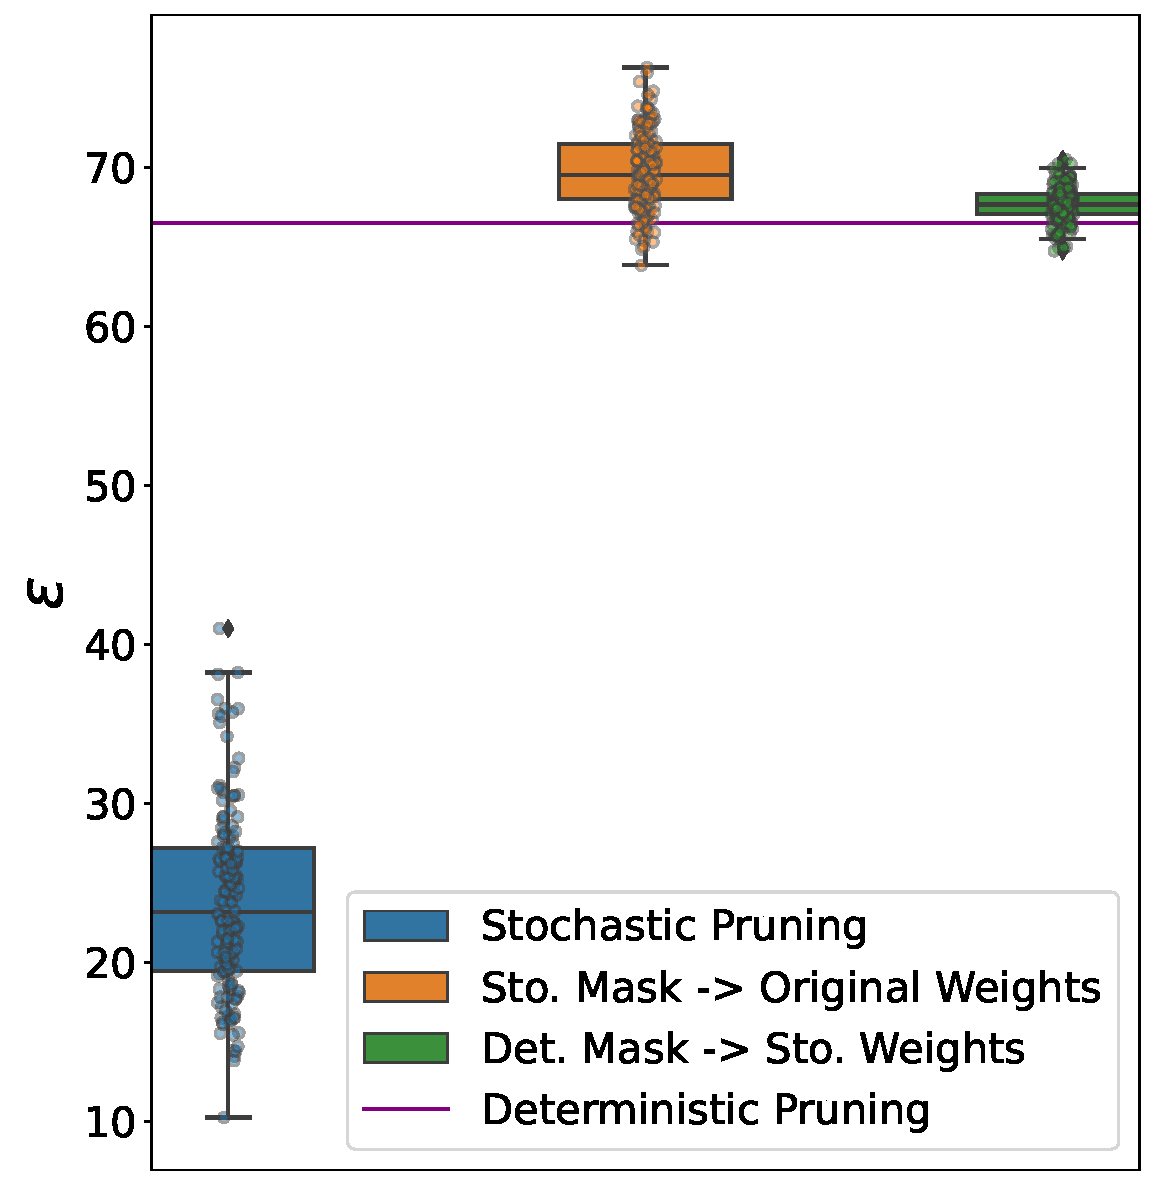
\includegraphics[width=\columnwidth]{figures/epsilon_allN_all_pr_0.9_sigma=0.005.pdf}
    % \caption{Accuracy degradation of One-shot Stochastic Pruning with $\sigma=0.001$ and pruning rate of 0.9} 
    \caption{Pruning rate 0.9} 
    \label{fig:pr0.9sigma0.005}
     \end{subfigure}
     \caption{Accuracy degradation of one-shot Stochastic Pruning and the resulting models of operations \ref{operation1} and \ref{operation2} with $\sigma=0.005$}
     \label{fig:sigma0.005}
\end{figure*}


In \cref{fig:stochastic_versus_deterministic} we observe that this simple operation, which we call \textit{Stochastic Pruning}, produces newly pruned networks that outperform the deterministic pruning of the original network in a one-shot scenario. 

%In \cref{fig:stochastic_versus_deterministic} we see how this simple operation in a one-shot manner already perform better than vanilla deterministic pruning. 
Inspired by \cite{zhouDeconstructingLotteryTickets2019}, where the authors claim that masking can be interpreted as a training procedure, we wanted to know if these newly discovered networks were better due to new weights or because they discovered better masks through \textit{Stochastic pruning}.
To measure this, we performed the following two operations.
\begin{enumerate}[label={\bfseries OP\arabic*}]
    \item We transfer the mask from noisy sparse models (pruned by our) to the original noiseless weights\label{operation1}
    \item We transfer the mask from the deterministic case to noisy weights. \label{operation2}
\end{enumerate}
If operation \ref{operation1} produces better models than deterministic pruning, it means that \textit{Stochastic Pruning} is capable of unveiling good masks and if operation \ref{operation2} produces better models than deterministic pruning, it means that the weights discovered by \textit{Stochastic Pruning}\todo{Should I mention stochastic pruning with italics and upper case every time or should I write it like that the first time an later just italics?}
are better than the original weights. In \cref{fig:pr0.8sigma0.001,fig:pr0.9sigma0.001,fig:pr0.8sigma0.005,fig:pr0.9sigma0.005} is the comparison of the accuracy degradation ($\epsilon$) for 160 noisy models for both operations for pruning rates of 0.8 and 0.9. Two main points can be concluded from these results; 1) \textit{Stochastic Pruning} can reveal a better mask for the original weights, but it is greatly affected by the pruning rate and noise level. 
Second, the deterministic mask combined with the noisy weights does not outperform the deterministic pruning of the original model for high levels of pruning. And finally, stochastic weights paired with the mask induced by magnitude pruning can reliably outperform deterministic pruning in the one-shot scenario. Note that the noise only reveals good subnetworks, since none of the dense stochastic networks outperforms the original dense network.

\subsection{Population Based Stochastic Pruning}
With this observation, we propose an iterative population-based algorithm that does not use fine-tuning for performance recovery. Our method is simple and more efficient than fine-tuning.
It is known that the distribution of the pruning rate per layer plays a significant role in the performance of sparse networks
\cite{leeLayeradaptiveSparsityMagnitudebased2022}. In this paper we use  the Erdös-Renyí-kernel distribution \cite{evciRiggingLotteryMaking2020} that has been proven to perform well in the random pruning regime\cite{liuUnreasonableEffectivenessRandom2022}. We prune each layer independently from each other.

\textbf{Noise level per layer:}
Since the statistics per layer differ from each other, we decided to use a different noise level ($\sigma$) for each one of them. In \cref{tab:Q50perLayer} are listed the medians of each layer. We decided to set the level of noise to the 10th percentile of the weight magnitude for each layer since we want to affect every layer uniformly.











\begin{algorithm}[tb]
   \caption{Bubble Sort}
   \label{alg:example}
\begin{algorithmic}
   \STATE {\bfseries Input:} data $x_i$, size $m$
   \REPEAT
   \STATE Initialize $noChange = true$.
   \FOR{$i=1$ {\bfseries to} $m-1$}
   \IF{$x_i > x_{i+1}$}
   \STATE Swap $x_i$ and $x_{i+1}$
   \STATE $noChange = false$
   \ENDIF
   \ENDFOR
   \UNTIL{$noChange$ is $true$}
\end{algorithmic}
\end{algorithm}
 
% We performed One-shot \textit{Stochastic Pruning} 160 times on an trained ResNet18 on CIFAR10 and transfer ed the stochastic mask into the original weights



%%%%%%%%%%%% In thi part I talk about how in this images for high pruning rates it seems that the combination of the stochastic weights is  better than the 

% In \cref{fig:OS0.001,fig:OS0.003,fig:OS0.005} can be seen the degradation in accuracy


% I wanted to know if these newly discovered networks were better due to new weights or whether they were better because better masks were found throughout the process.. For this,



% We were interested to know if this procedure was successful.



 % \missingfigure{This is a place holder figure}
%   This figure is to show that for one sample of one-shot pruning we can
%   outperform deterministic pruning for pruning rate 0.8
% \begin{figure}[htb]
%     \centering
%     \includegraphics[width=0.5\textwidth]
%     {transfers_comparison_gaussian_sigma_0.0021419609859022197_pr_0.8_batchSize_512_pop_10_t_14-29.pdf}
%     \caption{}
%     \label{fig:}
% \end{figure}\todo[inline]{Take the title away from ALL THE FIGURES}


  % \begin{figure}[htb]
  %   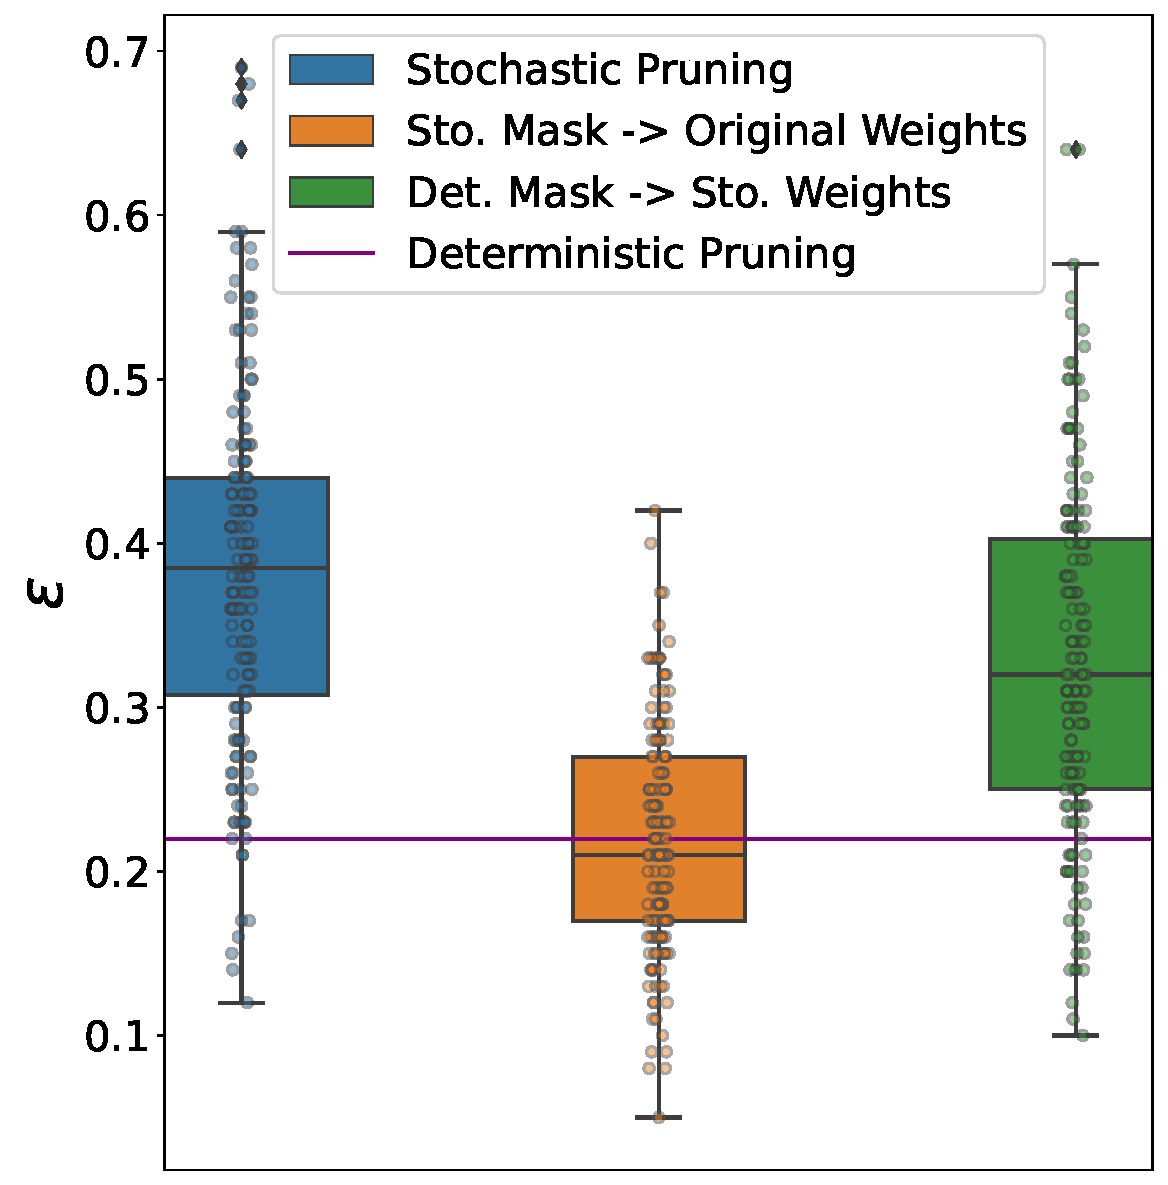
\includegraphics[width=\columnwidth]{figures/epsilon_allN_all_pr_0.5_sigma=0.003.pdf}
  %   \caption{Accuracy degradation on CIFAR10 for one-shot Stochastic Pruning with $\sigma=0.003$ and pruning rate of 0.5} \label{fig:pr0.5sigma0.003}
  % \end{figure}%
  % \begin{figure}[htb]
  %   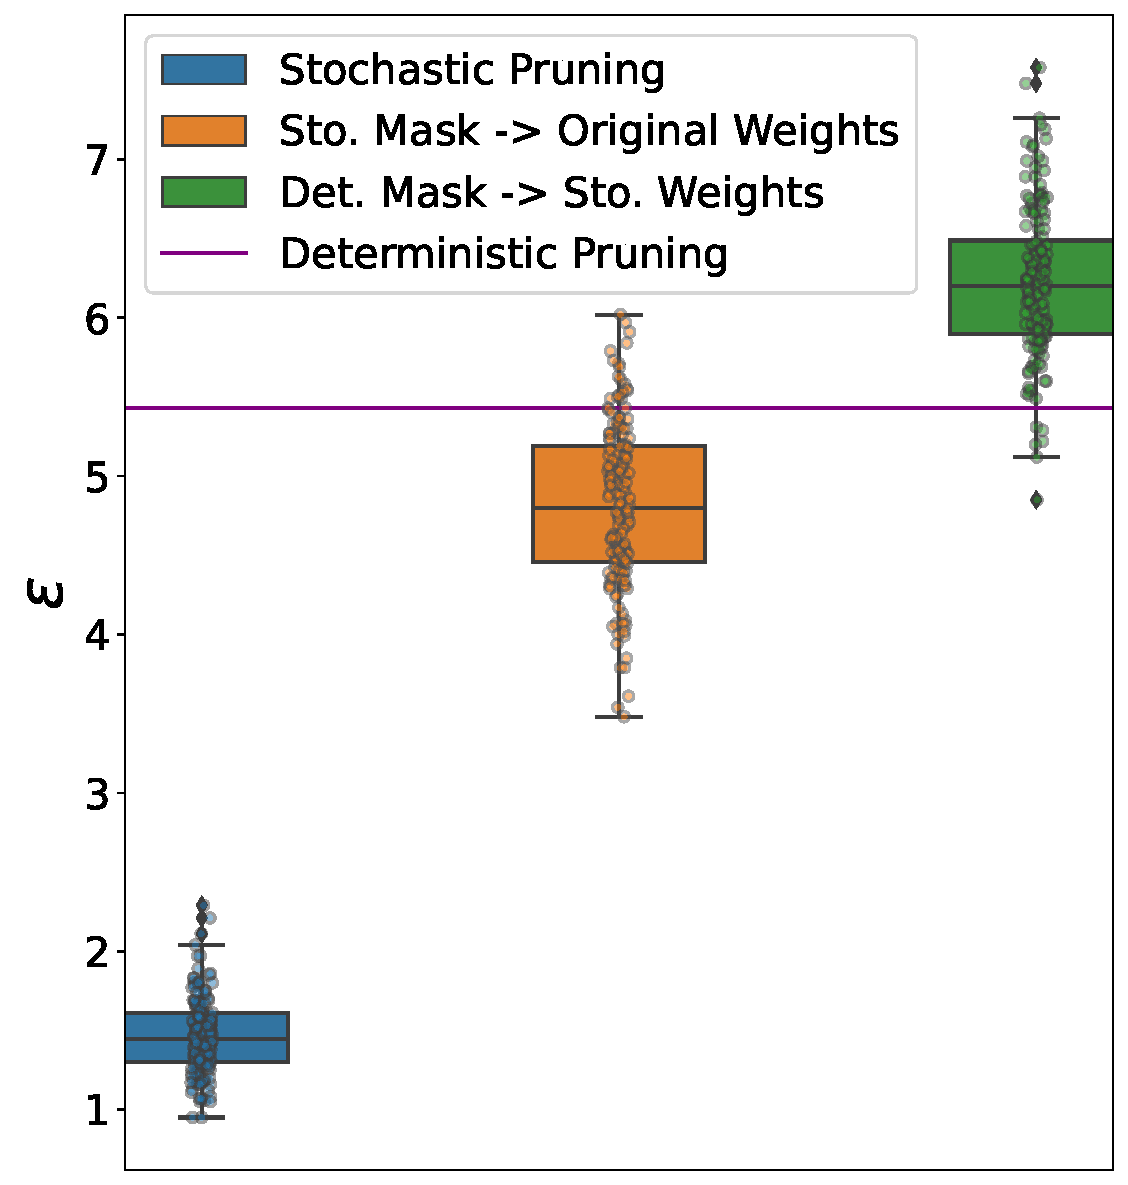
\includegraphics[width=\columnwidth]{figures/epsilon_allN_all_pr_0.8_sigma=0.003.pdf}
  %   \caption{Accuracy degradation on CIFAR10 for one-shot Stochastic Pruning with $\sigma=0.003$ and pruning rate of 0.8} \label{fig:pr0.8sigma0.003}
  % \end{figure}%
  % \hspace*{\fill}   % maximizeseparation between the subfigures
  % \begin{figure}[htb]
  %   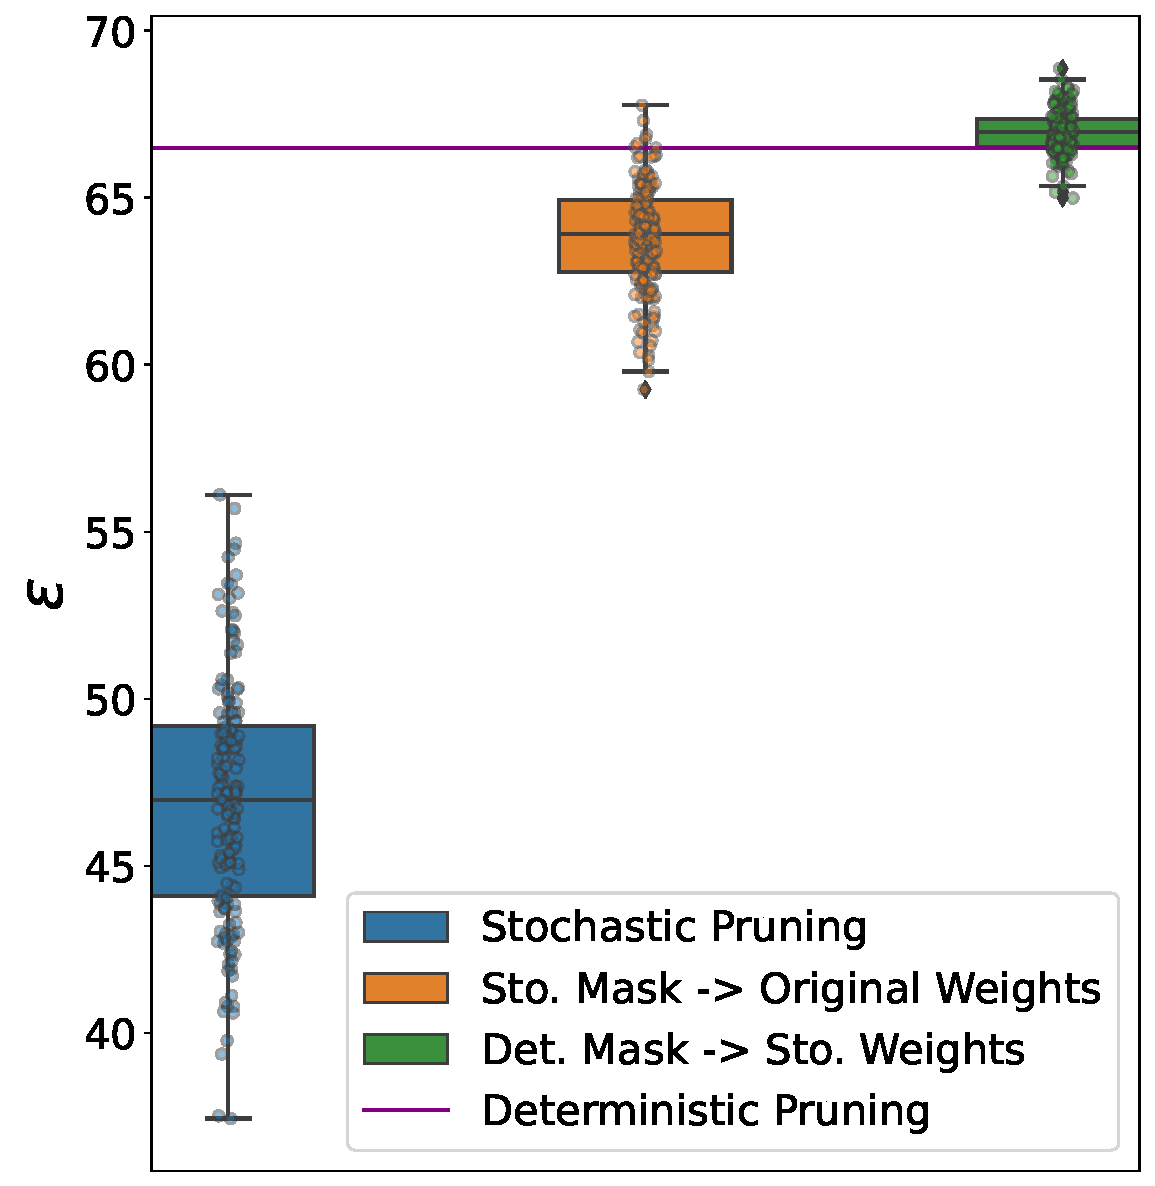
\includegraphics[width=\columnwidth]{figures/epsilon_allN_all_pr_0.9_sigma=0.003.pdf}
  %   \caption{Accuracy degradation of Stochastic Pruning wit $\sigma=0.003$ and pruning rate of 0.9} \label{fig:pr0.9sigma0.003}
  % \end{figure}














  
% \begin{figure}[htb]
%     \centering
%     \includegraphics[width=0.55\textwidth]{}
%     \caption{Accuracy degradation for one-shot stochastic pruning $\sigma=0.005$}
%     \label{fig:OS0.005}
% \end{figure}
  %\begin{figure}[ht]
  %    \centering
  %    \includegraphics[width=\columnwidth]
  %    {epsilon_allN_all_pr_sigma=0.001.png}
  %    \caption{Epsilon for $\sigma=0.001$ varying population size and different
  %    pruning rates}
  %    \label{fig:allNS0.001}
  %\end{figure}
  %\begin{figure}[ht]
  %    \centering
  %    \includegraphics[width=\columnwidth]
  %    {epsilon_allN_all_pr_sigma=0.003.png}
  %    \caption{Epsilon for $\sigma=0.003$ varying population size and different
  %    pruning rates}
  %    \label{fig:allNS0.003}
  %\end{figure}
  %\begin{figure}[ht]
  %    \centering
  %    \includegraphics[width=\columnwidth]
  %    {epsilon_allN_all_pr_sigma=0.005.png}
  %    \caption{Epsilon for $\sigma=0.005$ varying population size and different
  %    pruning rates}
  %    \label{fig:allNS0.005}
  %\end{figure}


%\section{Conclusions}




%%%%%%%%%%%%%%%%%%%%%%%%%%%%%%%%%%%%%%%%%%%%%%%%%%%%%%%%%%%%%%%%%%%%%%%%%%%%%%%
%%%%%%%%%%%%%%%%%%%%%%%%%%%%%%%%%%%%%%%%%%%%%%%%%%%%%%%%%%%%%%%%%%%%%%%%%%%%%%%
%  REFERENCES
%%%%%%%%%%%%%%%%%%%%%%%%%%%%%%%%%%%%%%%%%%%%%%%%%%%%%%%%%%%%%%%%%%%%%%%%%%%%%%%
%%%%%%%%%%%%%%%%%%%%%%%%%%%%%%%%%%%%%%%%%%%%%%%%%%%%%%%%%%%%%%%%%%%%%%%%%%%%%%%
%\nocite{*}
\bibliography{Pruning}
\bibliographystyle{icml2022}


%%%%%%%%%%%%%%%%%%%%%%%%%%%%%%%%%%%%%%%%%%%%%%%%%%%%%%%%%%%%%%%%%%%%%%%%%%%%%%%
%%%%%%%%%%%%%%%%%%%%%%%%%%%%%%%%%%%%%%%%%%%%%%%%%%%%%%%%%%%%%%%%%%%%%%%%%%%%%%%
% APPENDIX
%%%%%%%%%%%%%%%%%%%%%%%%%%%%%%%%%%%%%%%%%%%%%%%%%%%%%%%%%%%%%%%%%%%%%%%%%%%%%%%
%%%%%%%%%%%%%%%%%%%%%%%%%%%%%%%%%%%%%%%%%%%%%%%%%%%%%%%%%%%%%%%%%%%%%%%%%%%%%%%
\newpage
\appendix
\onecolumn
\section{ Appendix}
\subsection{Analysis of Stochastic Pruning per layer}

It could be the case that  stochastic pruning does not affect  all layers equally and the experiments show here  will tell us, which layers are more affected by stochastic pruning and if we should normalise the noise amplitude for each layer separately, given the distribution of their weight's magnitude

\begin{figure}[htpb]
    \begin{subfigure}{\textwidth}
    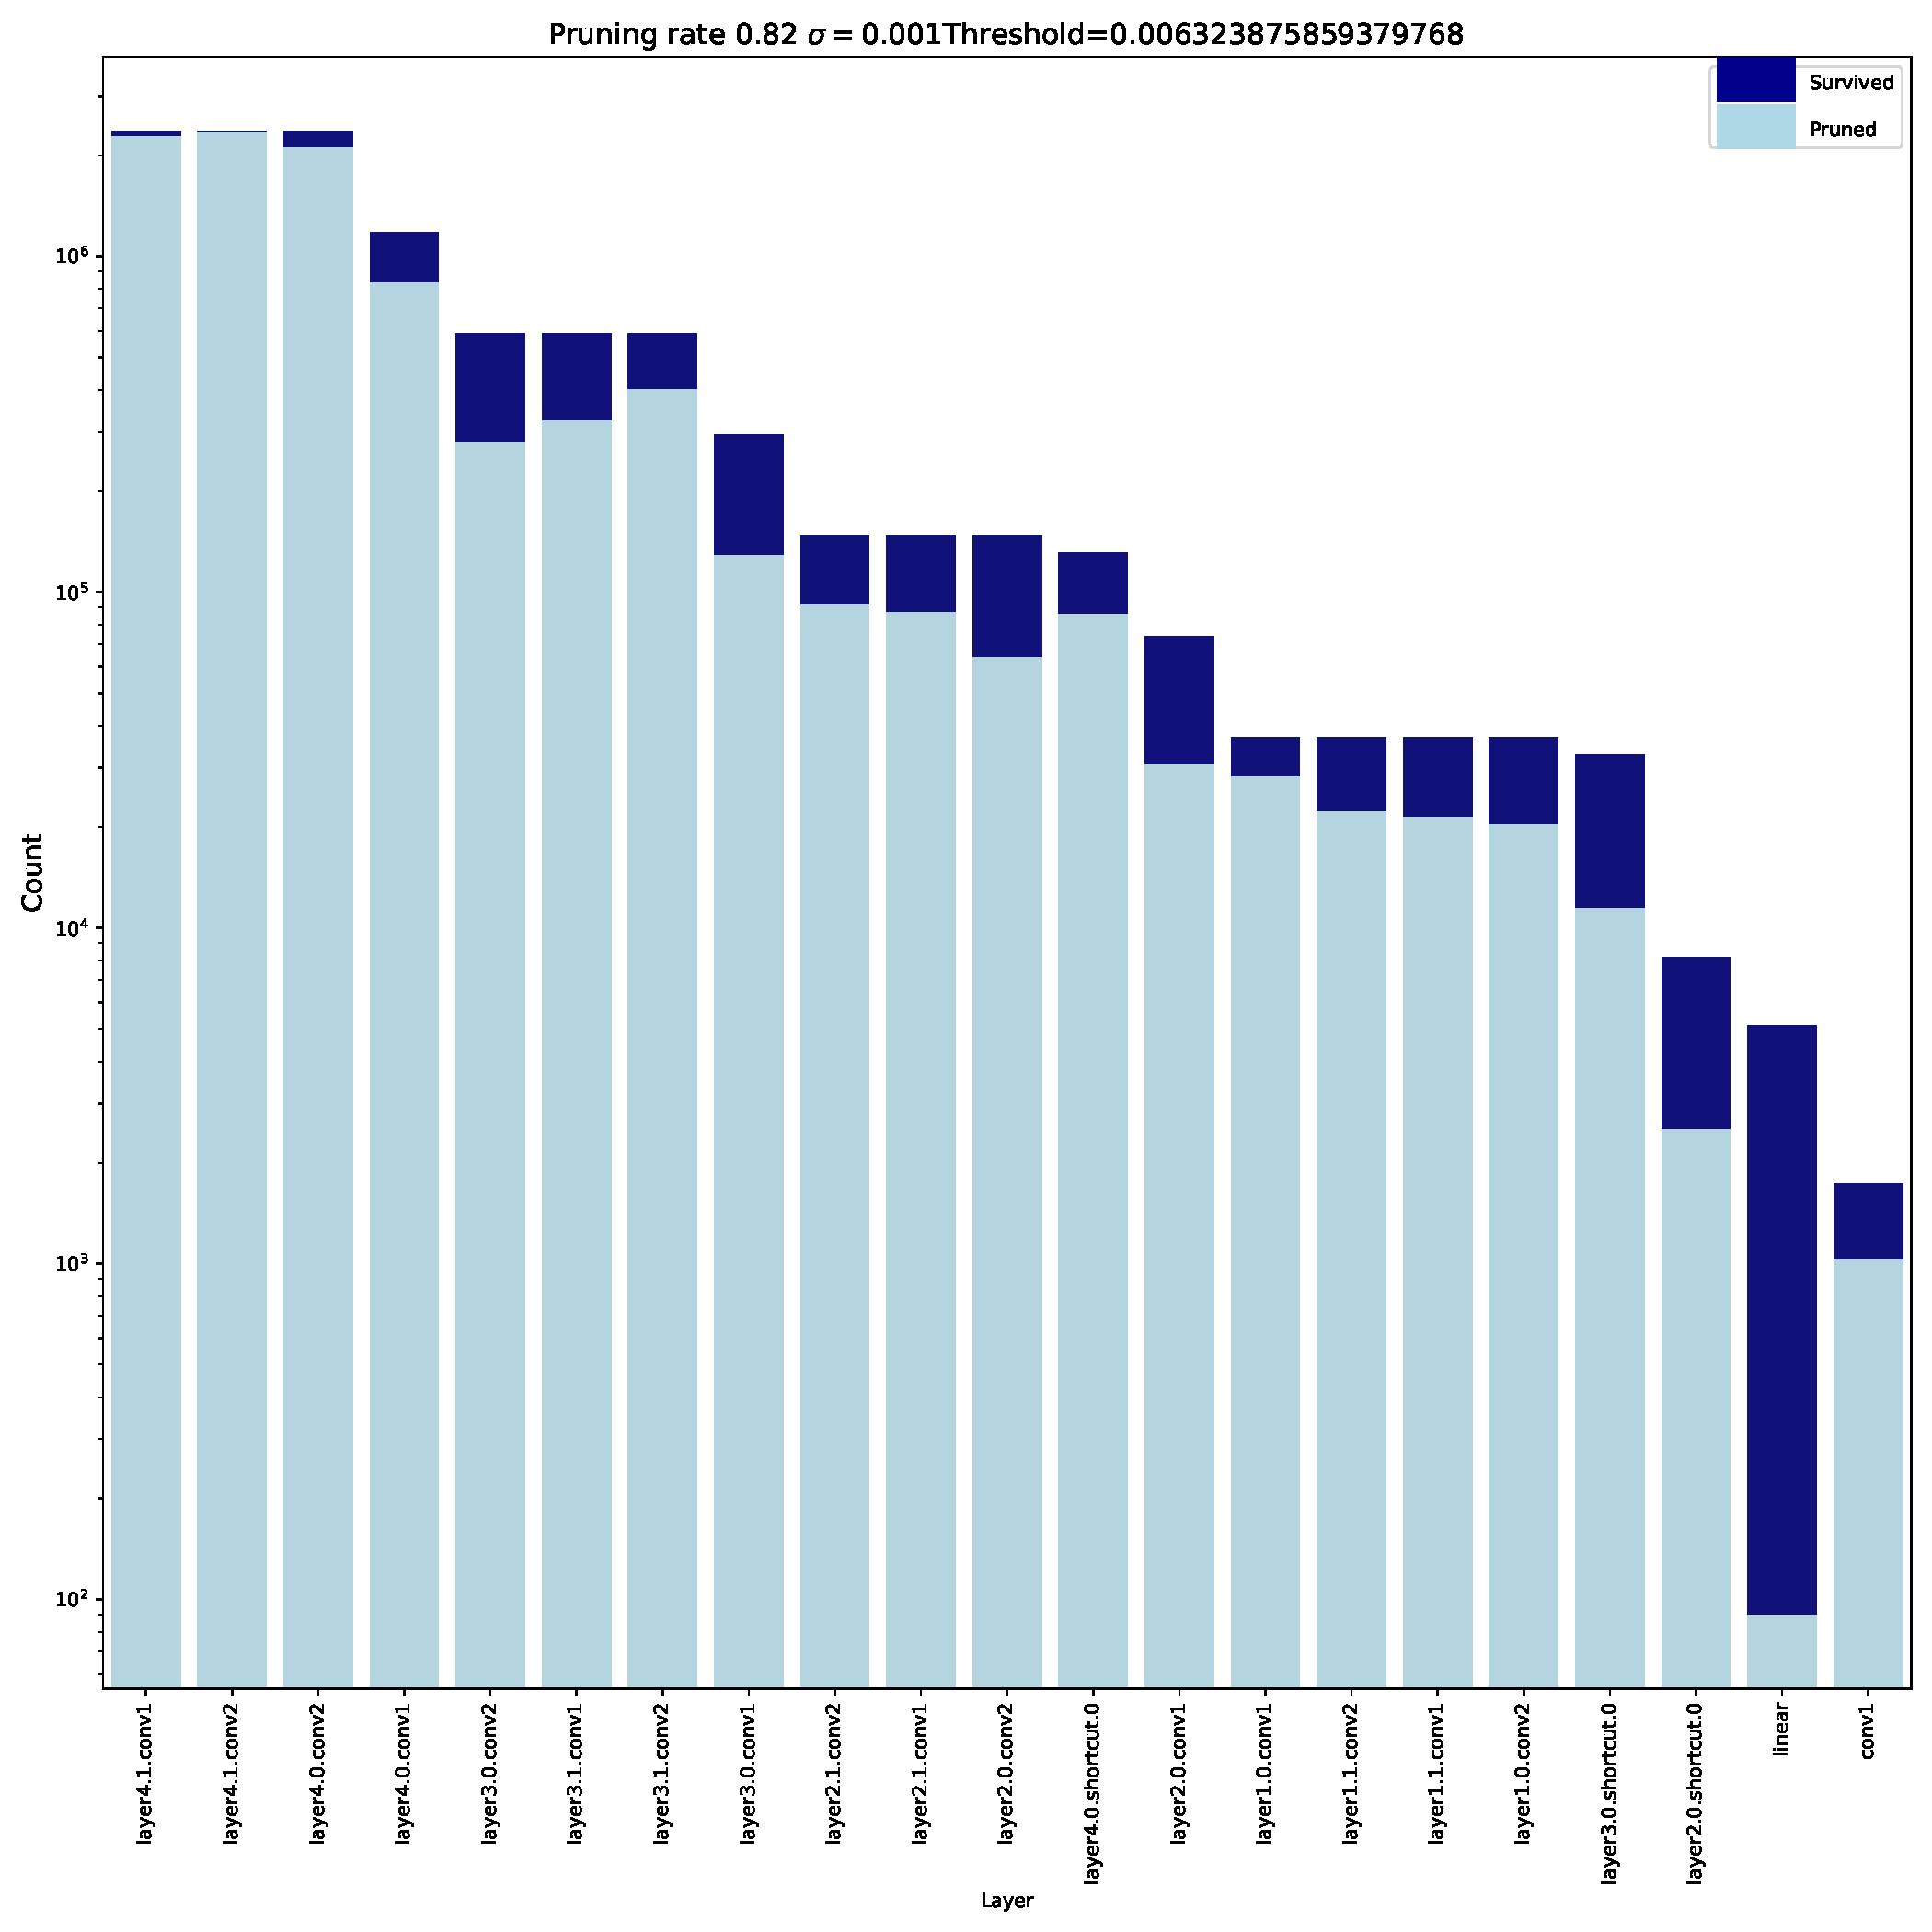
\includegraphics[width=0.4\textwidth]{supplementary/test_pr_0.82.pdf}
    \caption{Remaining and pruned weights for pruning rate 82\%}
    \label{subfig:pr_0.82}
    \end{subfigure}
    \hfill
    \begin{subfigure}{\textwidth}
    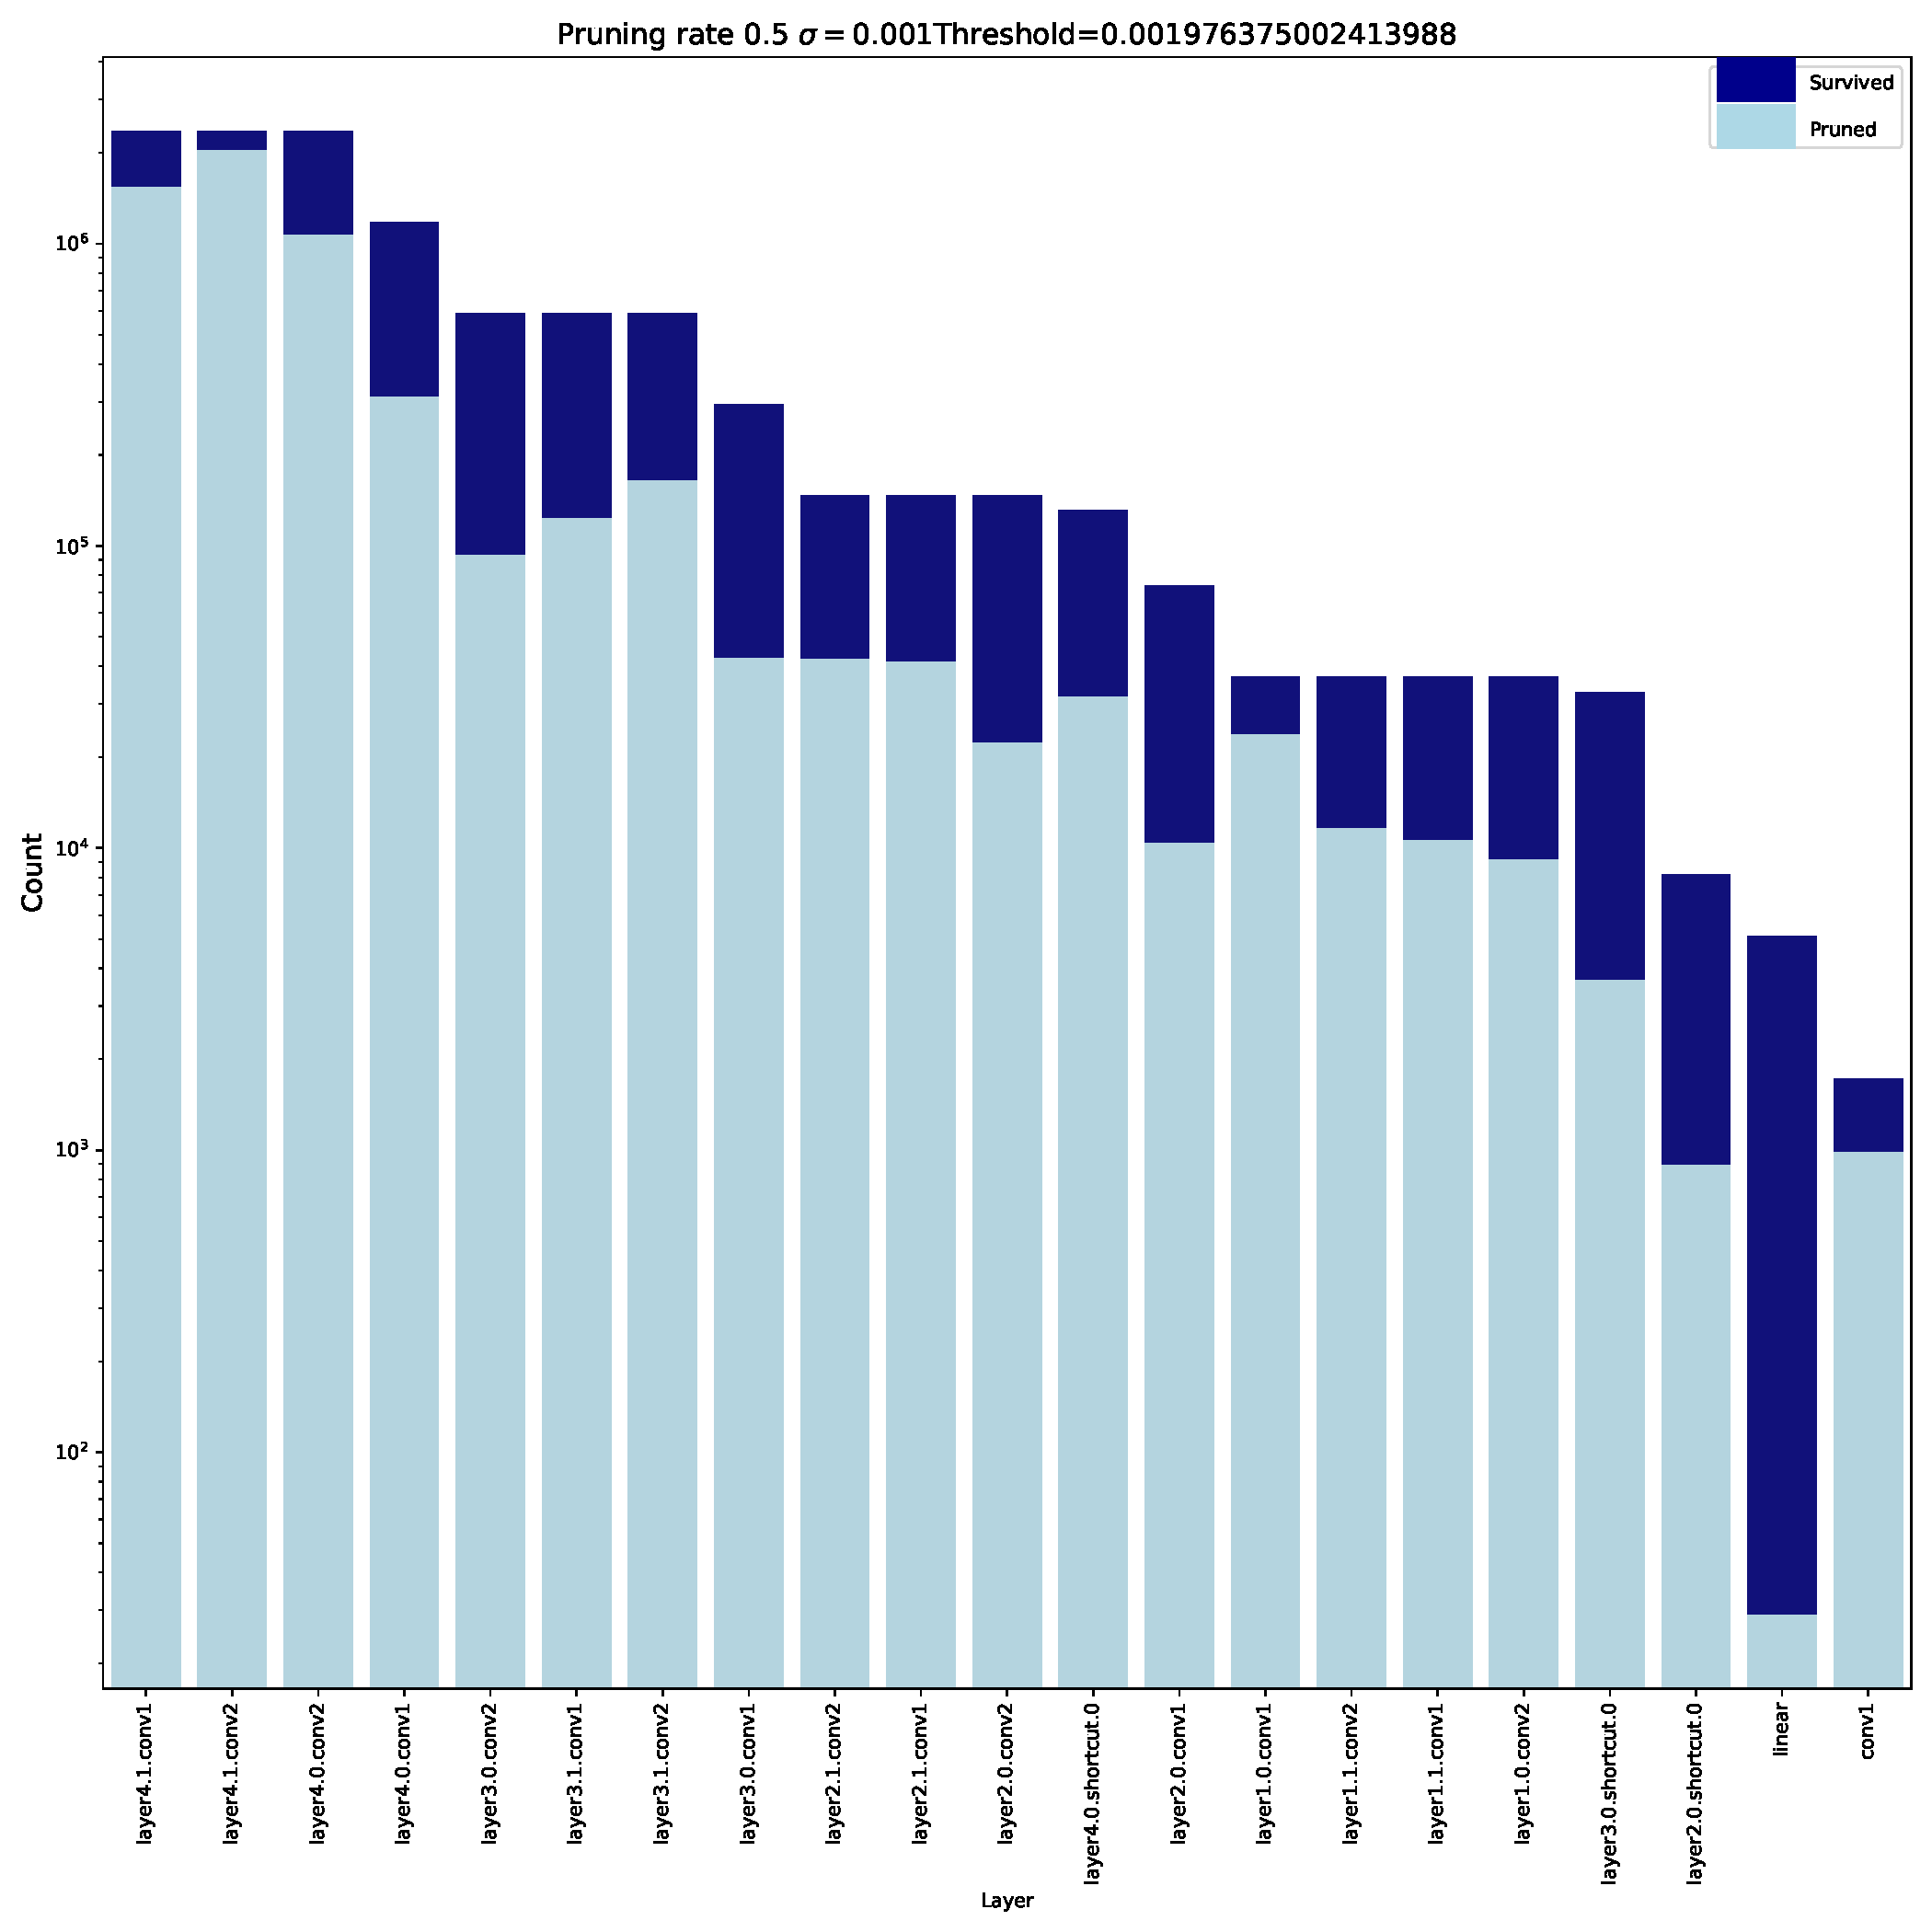
\includegraphics[width=0.4\textwidth]{supplementary/test_pr_0.5.pdf}
    \label{subfig:pr_0.5}
    \caption{Remaining and pruned weights for pruning rate 50\%}
    \end{subfigure}
    \hfill
    \begin{subfigure}{\textwidth}
    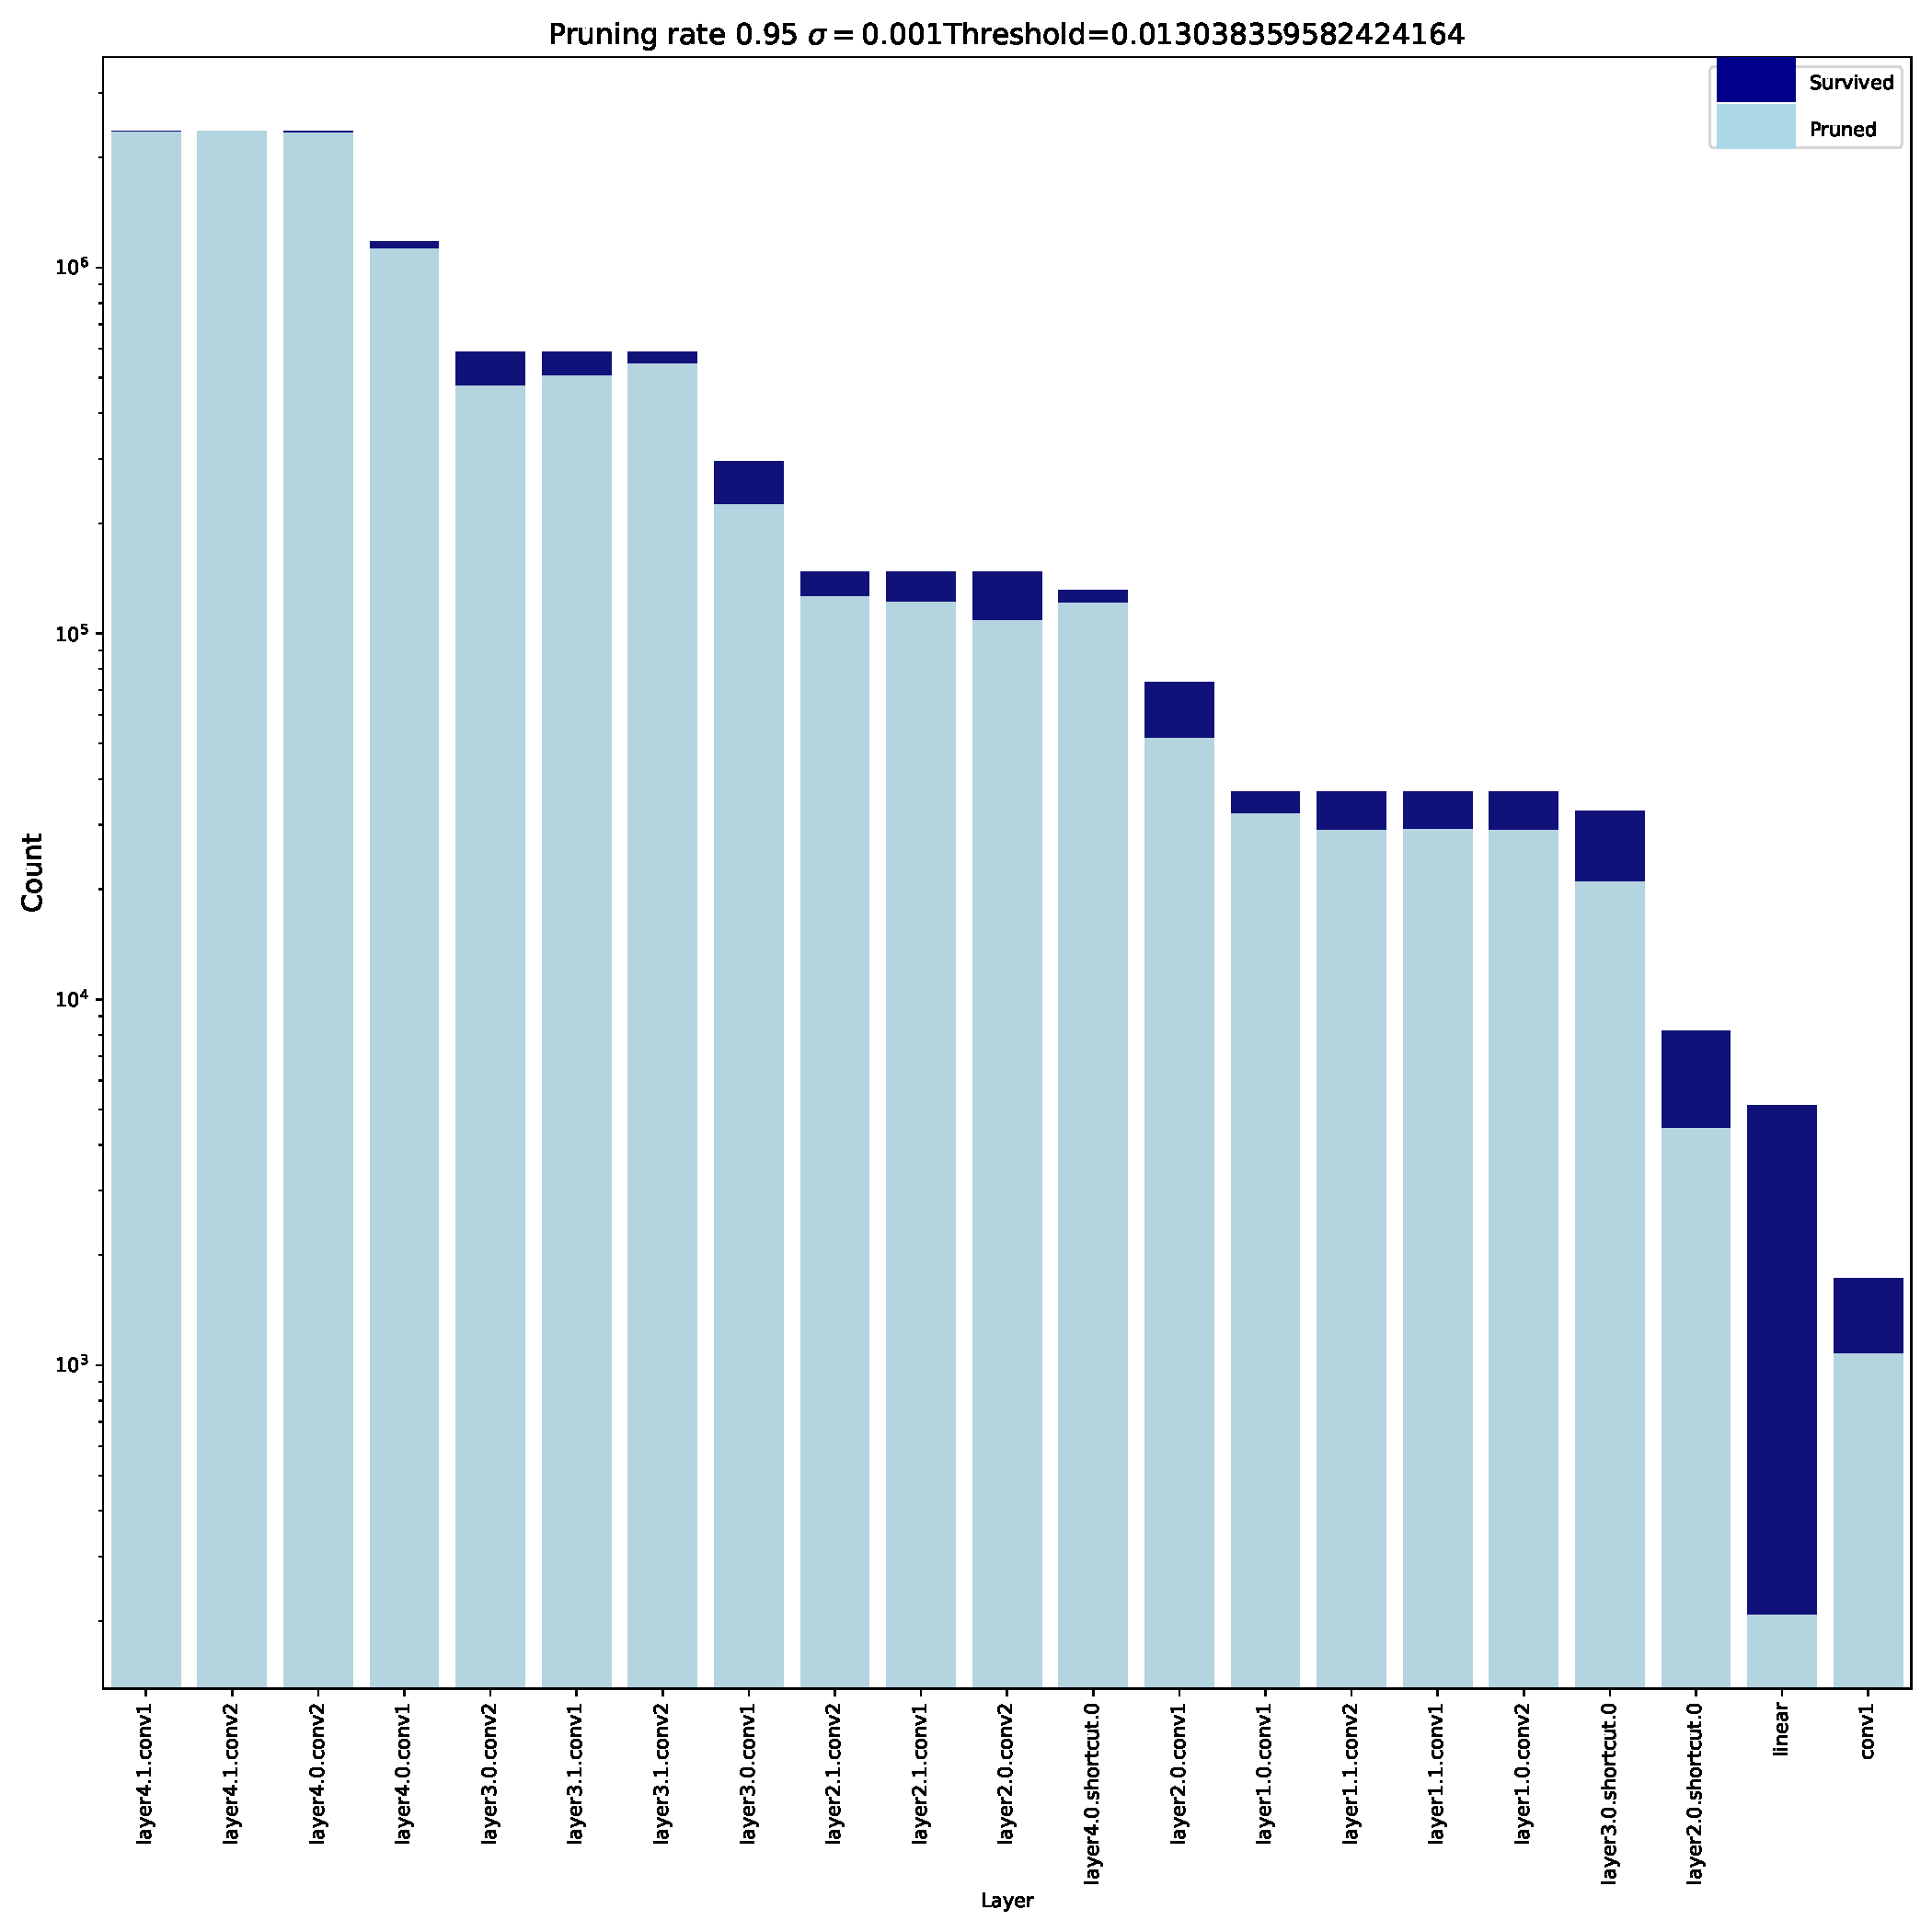
\includegraphics[width=0.4\textwidth]{supplementary/test_pr_0.95.pdf}
    \caption{Remaining and pruned weights for pruning rate 95\%}
    \label{subfig:pr_0.95}
    \end{subfigure}
    \hfill
    \caption{Survival and pruned weights by layer}
\end{figure}
Then


\end{document}


% This document was modified from the file originally made available by
% Pat Langley and Andrea Danyluk for ICML-2K. This version was created
% by Iain Murray in 2018, and modified by Alexandre Bouchard in
% 2019 and 2021 and by Csaba Szepesvari, Gang Niu and Sivan Sabato in 2022. 
% Previous contributors include Dan Roy, Lise Getoor and Tobias
% Scheffer, which was slightly modified from the 2010 version by
% Thorsten Joachims & Johannes Fuernkranz, slightly modified from the
% 2009 version by Kiri Wagstaff and Sam Roweis's 2008 version, which is
% slightly modified from Prasad Tadepalli's 2007 version which is a
% lightly changed version of the previous year's version by Andrew
% Moore, which was in turn edited from those of Kristian Kersting and
 Codrina Lauth. Alex Smola contributed to the algorithmic style files.
